\documentclass[11pt,a4paper]{article}

\usepackage{graphicx}
\usepackage{amsthm}
\usepackage{xcolor}
\usepackage{listings}
\usepackage{enumitem}
\usepackage{chngpage}
\usepackage[hidelinks]{hyperref}
\usepackage{listings}

\lstset{tabsize = 2}


\theoremstyle{definition}
\newtheorem{definition}{Definizione}[section]


\begin{document}
\title{Reti di Calcolatori a.a. 2019/2020}
\author{Francesco Iannelli}
\date{September 16, 2019}
\maketitle

\newpage
\tableofcontents
\newpage

\section{Introduzione al corso}
email: federica.paganelli@unipi.it\newline
modalità d'esame: prova scritta (compitini) e orale (facoltativo) più\newline
laboratorio che prevede progetto e orale. \newline
\underline{\textbf{N.B. Si accede alla prova orale di laboratorio solo dopo aver passato lo scritto.}}

\section{Cenni di modelli stratificati}
Sono architetture di comunicazione a strati. \newline
Concetti generali:
\begin{itemize}
	\item Stratificazione
	\item Information hiding
	\item Separation of concerns
\end{itemize}
Vantaggi della stratificazione:
\begin{itemize}
	\item \textbf{Facilità di progettazione.}
	\item \textbf{Facilità di manutenzione.}
	\item \textbf{Possibilità di riciclo.}
\end{itemize}
Due modelli: \textbf{ISO/OSI} (approccio top-down) e \textbf{Stack TCP/IP} (approccio bottom-up), quest ultimo vincente.\newline
Idea chiave: \underline{suddivisone in sottoproblemi.}
\begin{figure}[!h]
	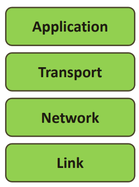
\includegraphics[scale=0.8]{Immagini/Modelli_Strat.png}
	\centering
	\caption{Modello stratificato}
\end{figure}

\pagebreak

\subsection{Livello applicativo}
Fanno parte del livello applicativo:
\begin{itemize}
	\item Identificativi delle risorse: URL, URI e URN.
	\item Il web: user agents, protocollo http.
	\item Protocollo FTP.
	\item TELNET: servizio di terminale virtuale.
	\item Posta elettronica.
	\item Sistema dei nomi DNS a dominio e la risoluzione dei nomi: iterativa e ricorsiva.
	\item molto altro ancora...
\end{itemize}

\subsection{Livello di trasporto}
Due tecnologie degne di nota:
\begin{enumerate}
	\item Protocollo \textbf{TCP}: \textbf{connection-oriented}, \textit{orientato alla connessione}.
	\item Protocollo \textbf{UDP}: \textbf{connection-less}, molto più leggero, prende dati applicativi e li affida allo strato IP, \underline{NON} da garanzie di consegna nè di ordine.
\end{enumerate}

\subsection{Livello rete}
Nel livello rete si ricava un percorso dall'host sorgente all'host destinatario usando le informazioni che si trovano nell'IP.\newline
Verrà trattato il protocollo Ipv4 e introdotto il protocollo Ipv6.

\subsection{Livello link}
Si occupa di gestire il collegamento tra due nodi \textbf{adiacenti}.
La tecnologia principale è l'\textbf{ethernet}.
\begin{figure}[!h]
	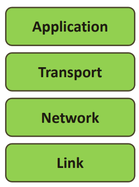
\includegraphics[scale=0.47]{Immagini/Modelli_Strat.png}
	\centering
	\caption{Modello stratificato}
\end{figure}
\pagebreak

\section{Introduzione alle reti}
\textit{Cos'è una rete? Quante tipologie di reti ci sono? Cos'è internet?}

\theoremstyle{definition}
\begin{definition}
	Una \textbf{rete} è un'interconnessione di dispositivi in grado di scambiarsi e interpretare le informazioni. Comprende sistemi terminali e intermedi: \textit{e.g. router, switch e modem.}
\end{definition}
I sistemi terminali si possono dividere in due tipi: \textbf{host} e \textbf{server}, sull'host girano le applicazioni utente mentre il server esegue programmi che forniscono servizi applicativi ad applicazioni. \newline \textit{N.B. il termine host può essere usato per indicare anche un server. \newline L'host, infatti, può essere sia un server sia il terminale di un utente che esegue un'applicazione client, più generalmente \textbf{l'host è una macchina}.}

\theoremstyle{definition}
\begin{definition}
	Una rete è formata da \textbf{dispositivi} e da \textbf{tecnologie}.
\end{definition}

\subsection{LAN}
Acronimo di \textbf{L}ocal \textbf{A}rea \textbf{N}etwork, è
una rete di area geografica limitata collegata attraverso una tecnologia ethernet \textbf{bus} o ethernet \textbf{switch}:
\begin{figure}[!h]
	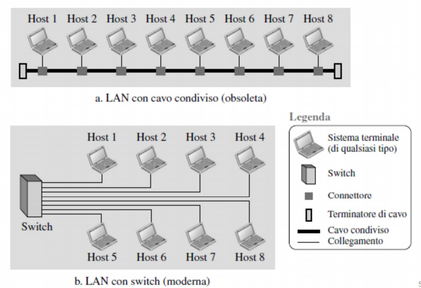
\includegraphics[scale=0.85]{Immagini/LAN.png}
	\centering
\end{figure}
Ciascun host ha un cavo che lo collega allo switch e a ogni porta dello switch corrisponde un host. Lo \textbf{switch} possiede una tecnologia di autoapprendimento ed è una componente del \textbf{livello link}.
\newpage

\subsection{WAN}
Acronimo di \textbf{W}ide \textbf{A}rea \textbf{N}etwork, è una rete di area geografica estesa: è composta da due o più reti collegate tramite un mezzo di trasmissione. Le reti coinvolte potrebbero anche essere reti LAN. \textit{(e il link potrebbe essere affittato a un'azienda da un operatore di telefonia).}
\begin{figure}[!h]
	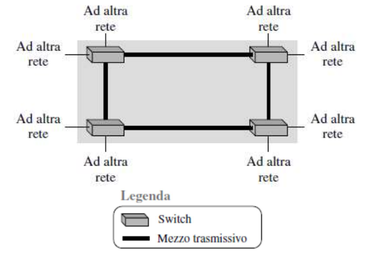
\includegraphics[scale=0.6]{Immagini/WAN_Switch.png}
	\centering
	\caption{Un esempio di WAN a cavo condiviso e a commutazione.\newline
		Queste WAN permettono l'esistenza di \textbf{percorsi alternativi} e la \textbf{divisione del traffico}. Una \textbf{WAN punto punto} invece ha \textbf{solo} 2 punti di terminazione.}
\end{figure}


\subsection{Internetwork}
L'internetwork è un sistema in cui ci sono più reti composte, capaci di scambiarsi informazioni e collegate. Concettualmente è una WAN ma è più complicata.\newline
I dispositivi che la compongono si distinguono in \textbf{sistemi terminali}
e dispositivi come gli \textbf{switch} e i \textbf{routers} che si trovano nel percorso tra i sistemi sorgente e i sistemi destinazione.
\begin{figure}[!h]
	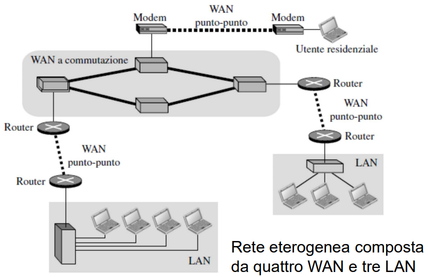
\includegraphics[scale=0.4]{Immagini/Internetwork.png}
	\centering
	\caption{Una internetwork.}
\end{figure}\newline
\textit{Problema: come mandare informazioni da un host a un altro?}


\subsubsection{Reti a commutazione di circuito}
Nelle \textbf{reti a commutazione di circuito} le \textbf{risorse} sono \textbf{riservate end to end} per ogni connessione. Risulta quindi necessario il \textbf{setup della comunicazione} per instaurare la connessione ed elargire le risorse.\newline
La risorsa non è tutto il link, bensì si considerano come risorse la capacità o la larghezza di banda porzionate per ogni connessione. Le risorse assegnate rimangono inattive se non utilizzate (\textit{e.g. telefonata}). I dispositivi mantengono lo stato della connessione. \textbf{Le performance sono garantite}. La capacità delle linee (\textit{link}) cambia a seconda della loro funzione all'interno della rete. Il \textbf{punto debole} delle reti a commutazione di circuito è la \textbf{poca flessibilità nel dispiegamento delle risorse}.


\subsubsection{Reti a commutazione di pacchetto}
Nelle \textbf{reti a commutazione di pacchetto} gli utenti inviano pacchetti che condividono le risorse del canale di comunicazione. \textbf{Non c'è} quindi \textbf{un canale dedicato} ai pacchetti di un singolo utente. La principale differenza rispetto alla commutazione di circuito risiede nell'implementazione della logica dei dispositivi di interconnessione, ovvero:
\begin{itemize}
	\item \textbf{Commutazione di Circuito}: avviene il \textbf{setup} della connessione dove  si prealloca l’utilizzo del collegamento trasmissivo con collegamenti
	      garantiti.
	\item \textbf{Commutazione di Pacchetto}: non viene instaurata una connessione bensì le informazioni necessarie si trovano all'interno dei pacchetti stessi, non ci sono informazioni di connessione memorizzate nei dispositivi coinvolti.
\end{itemize}
Nelle reti a commutazione di pacchetto quindi le risorse vengono usate a seconda della necessità. Possono quindi verificarsi situazioni di contesa delle risorse e sussiste il pericolo di congestione o di perdita dei pacchetti nel caso in cui la dimensione della coda del router non fosse sufficiente a contenere il flusso dei pacchetti entranti: il commutatore (\textit{router}) deve infatti ricevere l’intero
pacchetto prima di poter cominciare a trasmetterlo sul collegamento in uscita (\textit{\textbf{store and forward}}). \textbf{Non sono} quindi \textbf{garantite le prestazioni}.
\begin{figure}[!h]
	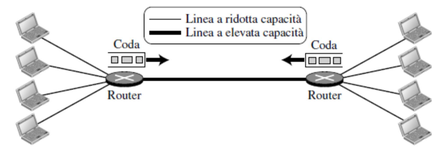
\includegraphics[scale=0.5]{Immagini/Packet_Switch.png}
	\centering
	\caption{Rete a commutazione di pacchetto. Da notare le diverse capacità dei link.}
\end{figure}
\newpage
\subsubsection{Packet Switch e Circuit Switch a confronto}
Vi sono 35 utenti su una rete con 100 Kbit/s di connessione e un link da 1 Mbit/s.
Ogni utente è attivo solo il 10\% del tempo.\newline
Con una \textbf{rete a commutazione di circuito} si riescono a gestire \textbf{solo} 10 utenti.\newline
Con una \textbf{rete a commutazione di pacchetto} si hanno i seguenti casi:
\begin{enumerate}
	\item 10 o meno utenti attivi: nessun problema.
	\item Più di 10 utenti attivi: ritardo.
\end{enumerate}
Tuttavia che gli utenti siano tutti e 35 attivi contemporaneamente è poco probabile (infatti $P(35) = 0.0004$).
Se ne deduce che la rete a commutazione di pacchetto riesce a gestire tutti gli utenti contemporaneamente nella maggior parte dei casi.

Nonostante il risultato ottenuto non si deve pensare che la rete a  commutazione di circuito sia obsoleta. Nel corso degli anni infatti le due tecnologie sono state \textbf{integrate} in vari modi.\newline
La commutazione di circuito infatti è usata nella telefonia fissa (\textit{PSTN: public switch telephone network}) per i servizi voce, la commutazione di pacchetto invece per i dati.\newline
Nelle reti ottiche di prima e seconda generazione si usano entrambe le tecnologie.

\subsubsection{Circuiti virtuali}
I circuiti virtuali funzionano nel seguente modo: viene stabilito un path tra host sorgente e host destinazione e tutti i pacchetti di un certo flusso seguono lo \textbf{stesso} path.
\subsubsection{Datagram Network}
Con \textbf{datagram} si indica un'entità informativa autocontenuta che contiene le informazioni sufficienti per essere indirizzata alla destinazione senza comunicazioni aggiuntive tra sorgente e destinazione: \textbf{non è quindi detto} che pacchetti di uno stesso flusso seguano lo stesso path sulla rete.
\newpage

\subsection{Internet}
\textit{Come interconnettere reti già esistenti?}\newline
\theoremstyle{definition}
\begin{definition}
	Una internet (con i minuscola) è una rete costituita da
	due o più reti interconnesse.
\end{definition}
La internet più famosa è chiamata \textbf{Internet} (con i maiuscola) ed è composta da migliaia di reti interconnesse. Ogni rete connessa ad Internet deve usare il protocollo IP e rispettare certe convenzioni su come vengono assegnati nomi e indirizzi.
Si possono facilmente aggiungere nuove reti. \newline Tuttavia è impensabile avere un link fisico tra ogni host, si hanno invece numerosi
dispositivi di interconnessione che permettono la comunicazione da un host all'altro e da un router all'altro.\newline
Uno scorcio delle \textbf{componenti di Internet}:
\begin{itemize}
	\item Miliardi di dispositivi interconnessi (e.g. hosts, end systems).
	\item Link di comunicazione (e.g. fibre ottiche, doppini telefonici,
	      cavi coassiali, onde radio).
	\item Routers: instradano pacchetti \textit{(sequenze)} di dati attraverso la rete.
\end{itemize}

\begin{figure}[!h]
	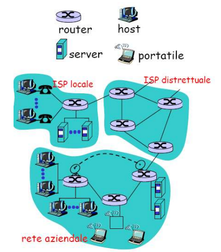
\includegraphics[scale=0.7]{Immagini/Internet.png}
	\centering
	\caption{Una porzione di Internet}
\end{figure}

Uno scorcio delle \textbf{entità software} di Internet:

\begin{itemize}
	\item Applicazioni e processi che elaborano le informazioni.
	\item \textbf{Protocolli} che regolamentano la trasmissione e la ricezione di informazioni e.g. TCP, IP, HTTP, FTP, PPP.
	\item Interfacce: verranno definite in seguito, sono le \textit{“membrane”} che separano gli \textit{"strati"}.
\end{itemize}

\subsubsection{Servizi}
L’\textbf{infrastruttura di comunicazione} consente il funzionamento delle applicazioni distribuite per scambio di informazioni \textit{(e.g. WWW, email, giochi, e-commerce, database, controllo remoto, ecc).}\newline
Lo \textbf{stack protocollare} offre il servizio di connessione. Vi sono due approcci:
\begin{enumerate}
	\item \textbf{Connection-less}: I dati vengono trasferiti \textbf{senza} stabilire una
	      connessione, non c'è nessuna garanzia di ordine e consegna. \textit{Ogni pacchetto ha una vita a sè.}
	\item \textbf{Connection-oriented}: Prevede l'\textbf{instaurazione della connessione}, il trasferimento dei dati e, in seguito, la chiusura della connessione. Garantisce integrità, completezza e ordine.
\end{enumerate}

\subsubsection{IETF/RFC/ICANN}

\theoremstyle{definition}
\begin{definition}
	L'IETF (Internet Engineering Task Force) è l’organismo che studia e sviluppa i protocolli in uso su Internet. Si basa su gruppi di lavoro a cui chiunque può accedere.
\end{definition}

\theoremstyle{definition}
\begin{definition}
	RFC/STD (Request For Comments \& STanDards) sono i documenti \textit{“ufficiali” } che descrivono i protocolli usati su Internet. Sono pubblicamente accessibili in rete.
\end{definition}

\theoremstyle{definition}
\begin{definition}
	ICANN (Internet Corporation for Assigned Names and Numbers) È un ente internazionale che coordina il sistema dei nomi di dominio (DNS), assegna i gruppi di indirizzi di rete, identificativi di protocollo e ha funzioni di controllo (blando) dello sviluppo di Internet.
\end{definition}

\subsubsection{Rete di accesso}
Internet è una internetwork che consente a qualsiasi utente
di farne parte. L’utente, tuttavia, deve essere fisicamente collegato a un
ISP (\textit{internet service provider}).
\theoremstyle{definition}
\begin{definition}
	Il collegamento che connette l'utente al primo router di internet è detto \textbf{rete di accesso}, suddetto collegamento può essere effettuato tramite rete telefonica, rete wireless o tramite accesso diretto.
\end{definition}

\newpage

\begin{figure}[!h]
	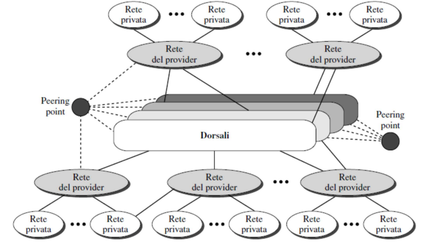
\includegraphics[scale=0.85]{Immagini/Internet_Concept.png}
	\centering
	\caption{Un modello concettuale di Internet}
\end{figure}

\section{Metriche di riferimento}
\textit{Come misurare le prestazioni di una rete?}\newline

\theoremstyle{definition}
\begin{definition}
	La \textbf{larghezza di banda} o \textbf{bandwidth} è la larghezza dell'intervallo di frequenze utilizzato dal sistema trasmissivo.
\end{definition}

\theoremstyle{definition}
\begin{definition}
	Il \textbf{bit rate} o \textbf{trasmission rate} è la quantità di dati che possono essere trasmessi o ricevuti nell'unità di tempo. [e.g. bps = bit/s]\newline
	Il bitrate dipende dalla tecnica trasmissiva ed è proporzionale alla larghezza di banda.
\end{definition}

\theoremstyle{definition}
\begin{definition}
	Il \textbf{throughput} è la quantità di traffico che arriva realmente a destinazione nell'unità di tempo, al netto di perdite sulla rete,
	del funzionamento dei protocolli etc.
\end{definition}

\theoremstyle{definition}
\begin{definition}
	La \textbf{latenza} o \textbf{latency} è il tempo che passa dal momento in cui il primo bit parte dalla sorgente al momento in cui l'intero messaggio arriva a destinazione. \newline
	\begin{center}
		\fbox{\Large{$L = r_{propagazione} + r_{trasmissione} + r_{accodamento} + r_{elaborazione}$}}
	\end{center}
\end{definition}
\newpage

\subsection{Ritardi}
Il ritardo introdotto da un nodo è la somma di questi 4 ritardi:
\begin{figure}[!h]
	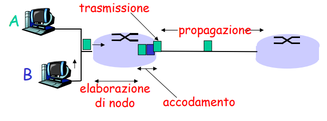
\includegraphics[scale=0.7]{Immagini/Ritardi.png}
	\centering
	\caption{Una visione di contesto}
\end{figure}

\subsubsection{Ritardo di elaborazione del nodo}
Il ritardo di elaborazione \textbf{è causato dall'elaborazione del percorso} (ovvero dove inoltrare il pacchetto scegliendo il percorso \textit{"migliore"}) \textbf{e dal controllo di errori sui bit}, è \textbf{tipicamente piccolo e trascurabile}.

\subsubsection{Ritardo di accodamento}
Il ritardo di accodamento \textbf{è il tempo che un pacchetto passa nella coda del router}, dipende dall'intensità e dal tipo di traffico. I pacchetti si accodano nei buffer dei router se il tasso di arrivo dei pacchetti eccede la capacità del collegamento di inoltrarli. Se non ci sono spazi liberi i pacchetti in arrivo vengono scartati.

\subsubsection{Ritardo di trasmissione}
Il ritardo di trasmissione \textbf{è il tempo impiegato a trasmettere un pacchetto intero} sul link.\newline
$R$ = rate di trasmissione del collegamento.\newline
$L$ = lunghezza del pacchetto.\newline
\[\centerline{$r_{trasmissione} = \frac{L}{R}$}\]
\subsubsection{Ritardo di propagazione}
Il ritardo di propagazione \textbf{è il tempo impiegato da un bit per essere propagato da un nodo (router) all'altro}.\newline
$d$ = lunghezza del collegamento fisico\newline
$s$ = velocità di propagazione del collegamento fisico \newline
\[\centerline{$r_{propagazione} = \frac{d}{s}$}\]

\subsection{Esempio}
Si consideri l'invio di un file di 1 MBit su un datalink di lunghezza 4800km:\newline
$d = 4800\times10^3 m$ \newline
$s = 3\times10^3 m/s$ \newline
Si calcoli il ritardo di propagazione. \newline
Soluzione:\newline\newline
$r_{propagazione} = \frac{d}{s} = \frac{4800\times10^3 m }{3\times10^3 m/s}  = 0.016$ secondi.\newline\newline
Sia il trasmission rate pari a 64 kbps, si calcoli il ritardo di trasmissione. \newline\newline
$r_{trasmissione} = \frac{L}{R} = \frac{10^6 bit}{64\times10^3 bps}= 15.625$ secondi.\newline\newline
Se il trasmission rate fosse invece di 1 Gbps? \newline\newline
$r_{trasmissione} = \frac{L}{R} = \frac{10^6 bit}{10^9 bps} = 0.001$ secondi.

\subsection{Volume di un link}
\begin{figure}[!h]
	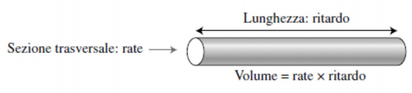
\includegraphics[scale=0.5]{Immagini/Link_Volume.png}
	\centering
\end{figure}
\theoremstyle{definition}
\begin{definition}
	Il volume di un link è il numero massimo di bit che il link può contenere.
\end{definition}
\centerline{\fbox{$Volume = bit rate\times ritardo$}}

\subsection{Esempio}
\begin{figure}[!h]
	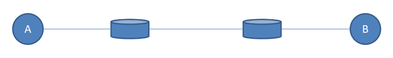
\includegraphics[scale=0.5]{Immagini/Esempio_ritardi.png}
	\centering
\end{figure}
Si calcoli il ritardo end-to-end di un pacchetto su un percorso con due router. Sia trascurabile il ritardo di congestione e si suppongano uguali su tutti link il propagation delay, il transmission delay e il processing delay.\newline\newline
\textbf{Soluzione}:\newline Essendoci due router intermedi bisongna attraversare tre link, quindi:\newline\newline
\centerline{$r_{totale} = 3\times r_{propagation} + 3\times r_{trasmission} + 3\times r_{processing}$}
\newpage
\begin{figure}[!h]
	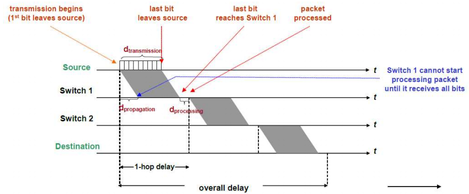
\includegraphics[scale=0.82]{Immagini/Soluzione_ritardi.png}
	\centering
	\caption{Quello che succede in dettaglio nell'esempio precedente.}
\end{figure}

\section{Modelli Stratificati e Protocolli}
\textit{Cos'è un protocollo? Cos'è uno strato?}

\begin{figure}[!h]
	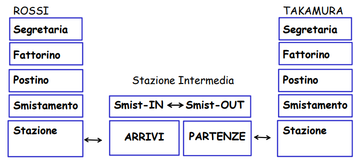
\includegraphics[scale=0.7]{Immagini/Postale.png}
	\centering
	\caption{Esempio di stratificazione. Si nota come i vari strati del modello interagiscono tra di loro, dal basso verso l'alto e viceversa, per consentire al sig. Rossi e al sig. Takamura di scambiarsi lettere.}
\end{figure}
\textbf{\underline{Vademecum per la lettura del seguente contenuto: N.B.}}:
\begin{enumerate}
	\item Gli strati comunicano \textit{(di solito)} \textbf{solo} con gli altri strati a loro adiacenti.
	\item Uno strato \textbf{fornisce} servizi allo strato superiore e \textbf{riceve} servizi da quello inferiore.
	\item La comunicazione tra strati adiacenti avviene attraverso un'\textbf{interfaccia}.
	\item Tra due entità diverse comunicano fra di loro solo gli strati dello \textbf{stesso livello} e secondo un \textbf{protocollo assegnato}, queste due entità sono dette \textbf{peer}.
\end{enumerate}
\newpage

\subsection{OSI: Open Systems Interconnection}
Le \textbf{prime} reti di calcolatori nacquero come \textbf{sistemi chiusi} in cui tutti i componenti dovevano essere dello stesso costruttore. Erano quindi tecnologie chiuse e \textbf{non interoperabili} l'una con l'altra a causa di drastiche differenze \textit{(e.g. differenza di linguaggio, \textbf{modelli di stratificazione diversi} e impossibilità per i programmi applicativi di riuscire ad operare in ambiente distribuito)}. Alla fine degli anni ‘60 esistevano: ARPANET, SNA (IBM), DNA (Digital).\newline
I \textbf{Sistemi Aperti} nascono dall'obbiettivo di alcune aziende di realizzare una rete di calcolatori in cui qualsiasi terminale potesse comunicare con un qualsiasi fornitore di servizi mediante qualsiasi rete.\newline\newline
Per realizzare un sistema aperto è necessario stabilire delle regole comuni: \textbf{gli standards}.
\theoremstyle{definition}
\begin{definition}
	Un sistema che implementa \textbf{protocolli aperti} è un \textbf{sistema aperto} (open system).
\end{definition}
\begin{definition}
	Un set di protocolli è \textbf{aperto} se:
	\begin{enumerate}
		\item I dettagli (\textbf{specifiche}) dei protocolli sono disponibili pubblicamente.
		\item I cambiamenti al set sono gestiti da un’organizzazione la cui
		      partecipazione è aperta al pubblico
	\end{enumerate}
\end{definition}

\subsubsection{Modello ISO/OSI}
L’International Organization for Standards (ISO) ha specificato
uno standard per l’interconnessione di sistemi aperti: l' \textbf{Open System Interconnection Reference Model} (OSI-RM) poi diventato standard internazionale nel 1983 (ISO 7498). \textbf{Si basa sul concetto di architettura a strati i cui criteri sono:}.
\begin{itemize}
	\item \textbf{Divisione delle funzionalità}: il protocollo di telecomunicazione è diviso in strati o layers, ognuno dei quali svolge un compito piccolo e indipendente dagli altri.\newline
	      Si cerca quindi di mantenere un minor numero di strati possibile e di far svolgere a ognuno di essi il minor numero di compiti possibile.
	\item \textbf{Comunicazione mediante interfacce}: i livelli comunicano mediante \textbf{chiamate standard}. Ogni livello è tenuto a rispondere alle \textbf{sole} chiamate che gli competono e che verranno
	      invocate dal singolo livello o dai due livelli ad esso adiacenti.
	\item \textbf{Information hiding}: le modalità con cui le funzioni competenti ad un livello
	      vengono svolte non è visibile dall'esterno che ne è così
	      svincolato.
\end{itemize}

\subsection{Protocollo}
\begin{figure}[!h]
	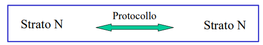
\includegraphics[scale=0.7]{Immagini/Protocollo.png}
	\centering
\end{figure}
I protocolli definiscono il \textbf{formato} e l’\textbf{ordine} dei
messaggi inviati e ricevuti tra entità della rete al livello n-esimo e
le \textbf{azioni} che vengono fatte per la loro \textbf{trasmissione} e
\textbf{ricezione}.
\theoremstyle{definition}
\begin{definition}
	Un \textbf{protocollo} è un insieme di regole che permettono a due entità uno scambio \textbf{efficace} ed \textbf{efficiente} delle informazioni. \textbf{Definisce} il \textbf{formato} e il
	\textbf{significato} dei frame (campi del messaggio), dei pacchetti o dei messaggi
	che vengono scambiati tra gli \textbf{strati paritari} di due
	entità diverse.
\end{definition}
Un protocollo specifica quindi:
\begin{itemize}
	\item La \textbf{sintassi} di un messaggio (e.g. i campi).
	\item La \textbf{semantica}.
	\item  \textbf{Le azioni da compiere }(e.g. per l'invio, alla ricezione, alla trasmissione etc...).
\end{itemize}
\theoremstyle{definition}
\begin{definition}
	Uno \textbf{strato} o livello è un modulo interamente definito attraverso i
	servizi, protocolli e le interfacce che lo caratterizzano.
\end{definition}
\theoremstyle{definition}
\begin{definition}
	Un' \textbf{interfaccia} è il set di regole governanti sintassi e semantica della comunicazione tra due \textbf{strati successivi} della \textbf{stessa entità}.
\end{definition}
\theoremstyle{definition}
\begin{definition}
	Un \textbf{servizio} è l'insieme di \textbf{primitive} (operazioni) che uno strato
	fornisce ad uno strato soprastante. (\textit{vedi sez. 3.4.1}).
\end{definition}
\begin{figure}[!h]
	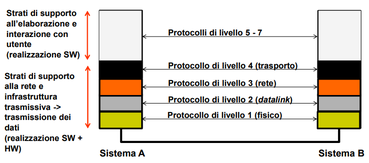
\includegraphics[scale=0.85]{Immagini/Protocol_stack.png}
	\centering
	\caption{Esempio di stack protocollare.}
\end{figure}
\begin{figure}[!h]
	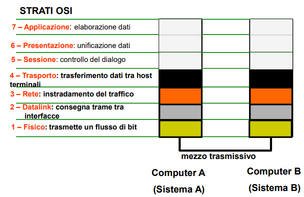
\includegraphics[scale=0.75]{Immagini/Osi_strati.png}
	\centering
	\caption{Gli strati di OSI.}
\end{figure}
\begin{figure}[!h]
	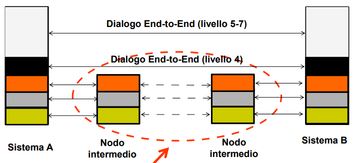
\includegraphics[scale=0.75]{Immagini/End_sys.png}
	\centering
	\caption{Esempio di collegamento tra end systems.}
\end{figure}
\newpage
\subsection{Incapsulamento dell'informazione}
All'interno della rete l'informazione ha origine \textbf{al livello
	applicativo} (\textit{livello 7 in figura}), discende quindi i vari livelli fino alla
\textbf{trasmissione}, che avviene mediante il \textbf{canale fisico}.
Da ogni livello attraversato viene aggiunta all'informazione una sezione informativa (o più di una) chiamata \textbf{header} che contiene informazioni pertinenti esclusivamente al livello stesso.
Per i dati ricevuti invece si segue il cammino inverso. Si tratta infatti di un \textbf{processo di incapsulamento \underline{reversibile}}.
\begin{figure}[!h]
	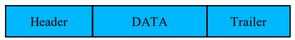
\includegraphics[scale=0.5]{Immagini/Incapsulamento.png}
	\centering
\end{figure}
\begin{itemize}
	\item \textbf{Header}: è la qualificazione del pacchetto dati per questo livello.
	\item \textbf{DATA}: è il payload proveniente dal livello superiore.
	\item \textbf{Trailer}: è usato per rilevare e correggere gli errori.
\end{itemize}

\begin{figure}[!h]
	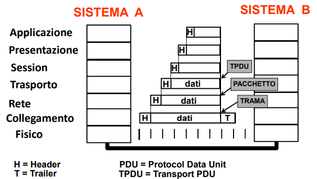
\includegraphics[scale=0.7]{Immagini/Incaps_2.png}
	\centering
	\caption{Il processo di incapsulamento. Da notare in particolare il payload.}
\end{figure}
\newpage

\section{Stack protocollare TCP/IP}
\textbf{TCP/IP} è una \textbf{famiglia di protocolli} attualmente
in uso su Internet.\newline Si tratta di una \textbf{gerarchia di
	protocolli} costituita da \textbf{moduli interagenti}, ciascuno dei
quali fornisce funzionalità specifiche.
Il termine \textbf{gerarchia} significa che ciascun protocollo di
\textbf{livello superiore} è supportato dai servizi \textbf{forniti} dai
protocolli di \textbf{livello inferiore}.
Definita in origine in termini di quattro livelli software
soprastanti a un livello hardware, \textbf{la pila TCP/IP} è \textbf{oggi}
intesa come \textbf{composta} \textbf{di cinque livelli}.
\begin{figure}[!h]
	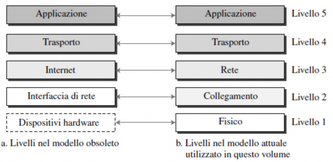
\includegraphics[scale=0.6]{Immagini/TCP_IP.png}
	\centering
	\caption{Livelli dello stack protocollare TCP/IP, si notino le differenze tra il modello originario e il modello attuale.}
\end{figure}
\begin{itemize}
	\item Il \textbf{livello applicativo} supporta le applicazioni di rete.
	\item Il \textbf{livello di trasporto} supporta il trasferimento di dati da un host all'altro.
	\item Il \textbf{livello di rete} instrada i datagrammi dalla sorgente alla destinazione.
	\item Il \textbf{livello link} trasferisce dati tra elementi adiacenti della rete.
	\item  Al \textbf{livello fisico} troviamo i bit sul link.
\end{itemize}
\begin{figure}[!h]
	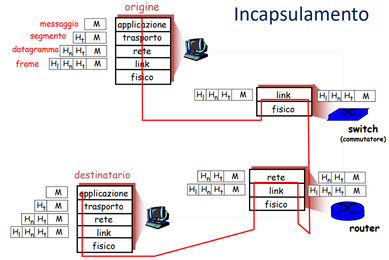
\includegraphics[scale=0.5]{Immagini/Incapsulamento_m.png}
	\centering
	\caption{Esemplificazione del processo di incapsulamento/decapsulamento dell'informazione.}
\end{figure}

\begin{figure}[!h]
	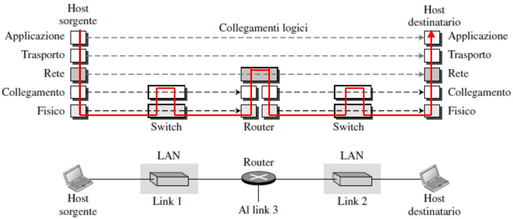
\includegraphics[scale=0.5]{Immagini/Logfis.png}
	\centering
	\caption{I vari collegamenti logici di comunicazione, in \textbf{rosso} invece, \textbf{il collegamento fisico}. La modularità del sistema fa in modo che gli strati paritari dei due host abbiano l'\textbf{illusione} di comunicare direttamente tra di loro. Si ricorda che queste entità situate a livelli corrispondenti su macchine (host) diverse sono dette \textbf{peer}.}
\end{figure}

\subsection{Lo strato applicativo}
Dello \textbf{strato applicativo} fanno parte le \textbf{applicazioni di rete}. Le applicazioni di rete sono composte da \textbf{processi distribuiti} e \textbf{comunicanti}, ovvero programmi eseguiti dai dispositivi terminali (host o end system) di una rete. Nella comunicazione \textbf{a livello applicativo} fra due dispositivi terminali interconnessi, due o più processi sono in esecuzione su ciascuno degli host comunicanti e si scambiano messaggi.
Il protocollo dello strato applicativo definisce: (\textit{repetita iuvant})
\begin{itemize}
	\item I \textbf{tipi} di messaggi scambiati al livello
	      applicativo (e.g. richiesta e risposta).
	\item La \textbf{sintassi} e la \textbf{semantica} dei campi dei messaggi.
	\item Le \textbf{regole} di comunicazione \textbf{interprocessuale}.
\end{itemize}
\begin{figure}[!h]
	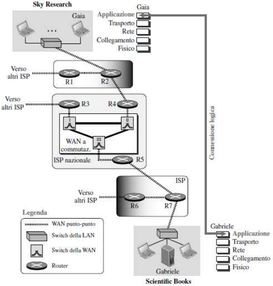
\includegraphics[scale=0.63]{Immagini/Application_layer.png}
	\centering
	\caption{Esempio di comunicazione tra applicazioni di rete. Ancora una volta è bene ricordare che il protocollo crea l'\textit{illusione} che i processi siano in comunicazione diretta.}
\end{figure}
Presentiamo ora i \textbf{paradigmi di comunicazione} dello strato applicativo:
\begin{itemize}
	\item \textbf{Client-Server}: prevede un numero \textit{limitato} di processi \textbf{server} che
	      offrono servizi e sono \textbf{sempre} in esecuzione in attesa di ricevere richieste dai client. Un \textbf{client} è un programma che richiede un servizio. Tipicamente il client inizia il contatto con il server \textbf{inviando una richiesta} e il server risponde \textbf{offrendo il servizio} richiesto.
	\item \textbf{Peer-to-Peer}: comunicazione tra \textbf{peer} \textit{(pari)} che possono sia \textbf{offrire} servizi che \textbf{inviare} richieste.
	\item  \textbf{Misto}.
\end{itemize}
\begin{figure}[!h]
	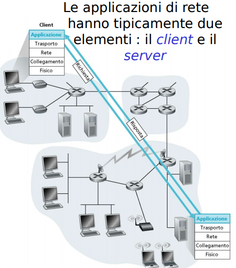
\includegraphics[scale=0.55]{Immagini/Client_server.png}
	\centering
	\caption{Esempio di paradigma client-server.}
\end{figure}
\newpage
Abbiamo, seppur assai brevemente, esaminato la comunicazione a livello applicativo tra macchine diverse. Scendiamo ora più nel dettaglio iniziando a tracciare il percorso \textbf{reale} dei dati dallo \textbf{strato applicativo} allo \textbf{strato di trasporto}. Partiamo dalla seguente definizione:

\theoremstyle{definition}
\begin{definition}
	\textbf{API}: acronimo di Application Programming Interface, è un insieme di \textbf{procedure} e \textbf{regole} che un programmatore deve seguire per accedere a delle risorse. Facilita molto la programmazione del software client-side.
\end{definition}
L' \textbf{API} che funge da \textbf{interfaccia} tra gli \textbf{strati di applicazione} \textbf{e} di \textbf{trasporto} è chiamata \textbf{socket} ed è usata dai processi dello strato applicativo per inviare e ricevere dati dallo strato di trasporto. Si tratta, ancora una volta, di una connessione \textbf{logica} poichè in realtà l'invio e la ricezione dei dati sono, nel \textbf{concreto}, responsabilità del sistema operativo e del protocollo TCP/IP.\newline
Riportiamo un estratto dell'\textbf{API} di \textbf{TCP:}\newline\newline
\texttt{connection TCPopen(IPaddress, int) //to open a conn.}\newline
\texttt{void TCPsend(connection, data) //to send data}\newline
\texttt{data TCPreceive(connection) //to receive data}\newline
\texttt{void TCPclose(connection) //to close a conn.}

\begin{figure}[!h]
	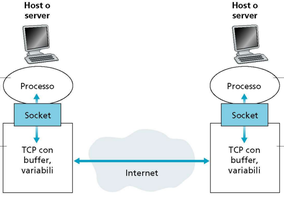
\includegraphics[scale=0.5]{Immagini/Socket.png}
	\centering
	\caption{In figura due processi che comunicano tramite socket. Il processo è controllato dallo sviluppatore dell'applicazione, tutto ciò che è presente sotto la socket è controllato dal sistema operativo.}
\end{figure}
Sorge ora spontanea una domanda: \textbf{se ci fossero più processi su ogni host}?\newline
Servirebbe un modo per \textbf{identificarli}... ci viene in aiuto il \textbf{socket address}.
\begin{figure}[!h]
	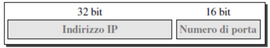
\includegraphics[scale=0.5]{Immagini/Socket_addr.png}
	\centering
	\caption{Il socket address identifica sia il \textbf{processo} con il numero di porta che l'\textbf{host} con l'indirizzo IP, a ogni porta corrisponde un processo.}
\end{figure}
\newpage
\textbf{\underline{Riassumendo}}: dello strato applicativo fanno parte le \textbf{applicazioni di rete}, composte da \textbf{processi distribuiti} su macchine diverse che comunicano tra di loro mediante il protocollo proprio dello strato applicativo. Sebbene il protocollo fornisca alle applicazioni l'illusione di comunicare direttamente, la comunicazione è in realtà garantita da tutto lo stack protocollare sottostante. In particolare, lo strato applicativo dipende dai servizi offerti dallo \textbf{strato di trasporto} che gli è immediatamente sottostante. I due strati comunicano tramite una \textbf{API} che si chiama \textbf{socket}.\newline\newline
A seconda del \textbf{servizio di trasporto richiesto} dall'applicazione è possibile che si trovino in uso \textbf{protocolli di trasporto diversi} tra i quali: \textbf{TCP} e \textbf{UDP}. \textit{(vedi sez. 2.2)}
\begin{figure}[!h]
	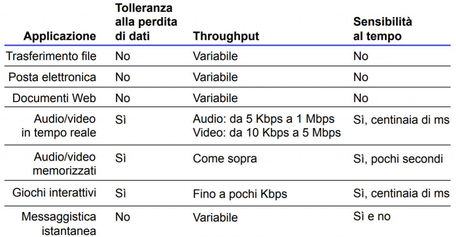
\includegraphics[scale=0.5]{Immagini/Tcp_udp.png}
	\centering
	\caption{In figura le caratteristiche di alcune delle principali applicazioni di rete. Non tutte le applicazioni sono uguali. Tipicamente la telefonia di internet usa il protocollo UDP.}
\end{figure}
\subsubsection{Web}
Il \textbf{web} è formato da risorse indirizzate da \textbf{URL}, acronimo di \textbf{uniform resource locator}. Generalmente queste risorse sono \textbf{pagine web}, formate da altri oggetti referenziati \textit{(e.g. altre pagine web, immagini ecc...)}. Lo \textbf{user agent} o \textbf{client} per il web è chiamato \textbf{browser} ed il \textbf{server} è chiamato \textbf{web server}.
\theoremstyle{definition}
\begin{definition}
	Una \textbf{URI} o Uniform Resource Identifier è una stringa compatta di caratteri che identifica una risorsa fisica o astratta.
\end{definition}
Le \textbf{URL} sono un \textbf{sottoinsieme} delle URI e identificano le risorse tramite la loro posizione all'interno della rete. Le \textbf{URN} acronimo di \textbf{uniform resource name} sono un altro sottoinsieme delle URI la cui funzione è di rimanere \textbf{globalmente uniche} e \textbf{persistenti} anche quando le risorse da loro puntate cessano di esistere o non sono più disponibili.
La \textbf{sintassi} delle URI è organizzata \textbf{gerarchicamente} e i componenti sono disposti in ordine di importanza da sinistra verso destra.
\begin{figure}[!h]
	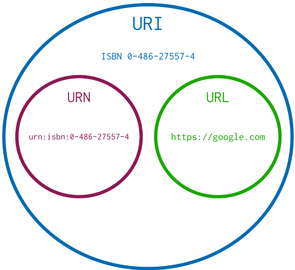
\includegraphics[scale=0.4]{Immagini/URIvsURL.png}
	\centering
	\caption{URN e URL non sono altro che specializzazioni delle URI.}
\end{figure}
\newpage
Le \textbf{sintassi} della URI:\newline\newline
\centerline{\LARGE$<scheme>://<authority><path>?<\textcolor{green}{query}>$}\newline\newline
\textcolor{red}{http}://\textcolor{blue}{maps.google.it}/\textcolor{purple}{maps}/\textcolor{purple}{place}?\textcolor{green}{q=largo+bruno+pontecorvo+pisa
	\&hl=it}
\begin{itemize}
	\item \textcolor{red}{\textbf{scheme}}: è \textbf{obbligatorio}, definisce lo \textbf{spazio dei nomi} della risorsa.
	\item \textcolor{blue}{\textbf{authority}}: indica il \textbf{nome di dominio} di un host \textit{(reg\_name)} o il suo \textbf{indirizzo IP} in notazione decimale puntata. Tipicamente identifica un computer sulla rete.
	\item \textcolor{purple}{\textbf{path}}: contiene \textbf{dati} specifici per l’authority (o per lo scheme) e \textbf{identifica} la risorsa \textbf{nel contesto} di quel namespace e di quell'authority.
\end{itemize}
Le URI possono essere \textbf{assolute} o \textbf{relative}, una \textbf{URI assoluta} identifica una risorsa \textbf{indipendentemente} dal contesto in cui è usata. Una \textbf{URI relativa} identifica una risorsa in relazione ad un'altra URL, \textbf{è priva di schema e di authority}, non viaggia sulla rete ed è interpretata dal browser in relazione al documento di partenza.\newline \textit{(e.g. http://www.w3.org/pub/WWW/TheProject.html oppure\newline /pub/WWW/TheProject.html \underline{sotto l'host}: www.w3.org)}.
\subsubsection{HTTP Protocol}
\label{sec:HTTP Protocol}
Il protocollo \textbf{HTTP} è un protocollo di tipo \textbf{request}/\textbf{response}: il client inizia la connessione inviando un messaggio di \textbf{request} al server che a sua volta invia una \textbf{response}. Si tratta di un \textbf{protocollo generico}, poichè non dipende dal formato delle risorse, e \textbf{stateless} poichè \textbf{le coppie richiesta/risposta sono indipendenti l'una dall'altra}. In \textbf{HTTP 1.0} dopo la prima coppia di richiesta/risposta la connessione viene \textbf{terminata} mentre in \textbf{HTTP 1.1} si \textbf{procede} con un’altra coppia. \newline
Lo \textbf{schema http} è usato per accedere alle risorse attraverso il protocollo HTTP. \newpage
Si riporta di seguito la \textbf{sintassi} per le URL http:\newline\newline
\centerline{\LARGE$http: // <host> [ : <port> ] [ <path> ]$}
\begin{itemize}
	\item \textbf{host}: è un \textbf{host domain di Internet} valido oppure un indirizzo IP in forma decimale puntata.
	\item \textbf{port}: \textbf{è un intero}, se  la porta è vuota o non è indicata si usa automaticamente la porta 80.
	\item \textbf{path}: specifica la \textbf{request URI} \textit{(vedi seguito)}.
\end{itemize}
\textbf{\underline{N.B.} Il protocollo HTTP utilizza il protocollo TCP tramite la sua API.}\newline\newline
//esempio client\newline
\texttt{c = TCPopen("131.115.7.24", 80);}\newline
\texttt{TCPsend(c,"GET /index.html");}\newline
\texttt{d = TCPreceive(c);}\newline\newline
\texttt{//esempio server}\newline
\texttt{p = TCPbind(80); //where to wait for connections}\newline
\texttt{d = TCPaccept(p); //waiting for connections}\newline
\texttt{r = TCPreceive(d);}\newline
\texttt{...}\newline
\texttt{TCPsend(d,pag);}\newline
\texttt{TCPclose(d);}\newline
\theoremstyle{definition}
\begin{definition}
	Una \textbf{connessione http} è  un circuito logico di livello di trasporto stabilito tra due programmi applicativi per comunicare tra loro.
\end{definition}
Una \textbf{connessione} può essere:
\begin{itemize}
	\item \textbf{Non persistente}\textit{(http1.0: RFC 1945)}: si parla di connessione non persistente quando \textbf{per ogni richiesta} del \textbf{client} viene instaurata \textbf{una nuova connessione} con il \textbf{server}. Ciò aumenta il \textbf{carico} su quest ultimo e potrebbero verificarsi fenomeni di \textbf{congestione}. \textit{Infatti per visualizzare le n immagini di un sito il client invia di seguito n richieste al server.}
	\item \textbf{Persistente}\textit{(http1.1: RFC 2616)}: la connessione è appunto \textbf{persistente}. Nello \textbf{standard} è specificato un meccanismo che consente al server di \textbf{chiudere} la connessione TCP su richiesta del client. \textit{(CONNECTION = CLOSE, in GENERAL HEADER, vedi seguito.)}\newline \textbf{\underline{N.B.}} Una volta che la chiusura della connessione è stata segnalata, il client \textbf{non deve} inviare altre richieste.
\end{itemize}
\newpage
\textbf{Esempio:}\newline
Supponiamo che l’utente digiti la seguente URL:\newline\newline \centerline{\textbf{www.someSchool.edu/someDepartment/home.index}}\newline\newline
Con \textbf{una connessione non persistente}, in ordine temporale succedono le seguenti cose:
\begin{enumerate}
	\item Il \textbf{client http}  invia una richiesta di connessione
	      \textbf{TCP} verso il server http al \textbf{www.someSchool.edu} \textit{(La porta 80 è usata di default per il server http.)}
	\item Il \textbf{server http} dell’host	\textbf{www.someSchool.edu}, che aspetta le richieste di connessione \textbf{TCP} alla \textbf{porta 80}, \textbf{accetta} \textbf{la richiesta di connessione}  e notifica il client.
	\item Il \textbf{client http} invia quindi un \textbf{messaggio di richiesta}, contenente la URL.
	\item Il \textbf{server http} riceve il messaggio di richiesta, compila un \textbf{messaggio di risposta} con l’oggetto richiesto indicato dalla URL: \textbf{someDepartment/home.index}, invia il messaggio e in seguito \textbf{chiude} la connessione.
	\item Il \textbf{client http}  riceve il messaggio di risposta che contiene il file html e lo visualizza.
\end{enumerate}
\textit{Si ricorda che la ricezione e la trasmissione di tutti i messaggi elencati poco sopra avviene tramite socket.}\newline
Supponiamo ora che la URL contenga dei riferimenti a 10 immagini, in tal caso per ogni riferimento si devono ripetere tutti i passaggi definiti sopra. Salta immediatamente all'occhio la \textbf{scarsa efficienza} della procedura.\newline\newline
Con \textbf{una connessione persistente} invece il server lascerebbe aperta la connessione TCP dopo aver spedito la prima risposta e vi riceverebbe quindi le richieste successive. La connessione verrebbe chiusa dal server quando specificato nell’header di un messaggio  \textbf{inviatogli dal client}, oppure alla mancata ricezione di richieste per un certo intervallo di tempo \textit{(time out)}.\newline\newline
Un ulteriore miglioramento delle prestazioni, si otterrebbe con una tecnica di \textbf{pipelining}, consistente nell’invio da parte del client di molteplici richieste senza aspettarne la ricezione da parte del server.\newline
Il \textbf{server} \textbf{deve} tuttavia inviare le risposte nello stesso ordine in cui sono state ricevute le richieste e il \textbf{client} \textbf{non} può inviare \textbf{in pipeline} richieste che usano metodi HTTP \textbf{non idempotenti}. Ma cos'è un \textbf{metodo idempotente}?
\theoremstyle{definition}
\begin{definition}
	Un \textbf{metodo idempotente} è un metodo tale che il suo effetto collaterale sulla risorsa è lo \textbf{stesso} per N o 1 richieste identiche che ne fanno uso. \textit{(e.g. GET, HEAD, PUT, DELETE, OPTIONS, TRACE)}
\end{definition}
\theoremstyle{definition}
\begin{definition}
	Un \textbf{metodo safe} è un metodo che non produce effetti collaterali sulle risorse. \textit{(e.g. non le modificano: GET, HEAD, OPTIONS, TRACE...)}
\end{definition}
\begin{figure}[!h]
	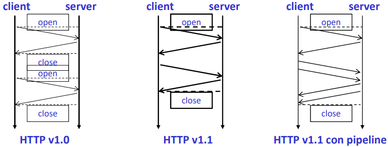
\includegraphics[scale=0.85]{Immagini/Http_vs.png}
	\centering
	\caption{In figura sono rappresentate le differenze viste prima.}
\end{figure}
\textit{Come sono strutturati i messaggi HTTP?}\newline\newline
Riportiamo di seguito la \textbf{struttura} di un generico messaggio http:\newline
\texttt{Request = Request-Line} \textit{o} \texttt{Response = Status-Line} \textit{per i messaggi di risposta.}\newline
\texttt{*( general-header}\newline
\texttt{| request-header} \textit{o} \texttt{response-header}\newline
\texttt{| entity-header )}\newline
\texttt{CRLF}\newline
\texttt{[ message-body ]}\newline
La prima riga o \textbf{start line} distingue i messaggi di request dai messaggi di response.
\begin{figure}[!h]
	\centering
	\begin{minipage}[b]{0.4\textwidth}
		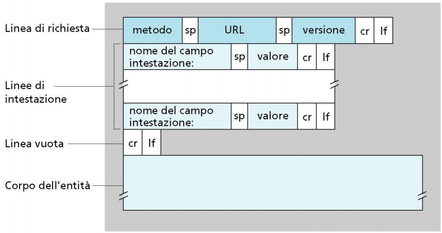
\includegraphics[scale=0.4]{Immagini/Http_req.png}
		\caption{In figura un messaggio di richiesta.}
	\end{minipage}
	\hfill
	\begin{minipage}[b]{0.4\textwidth}
		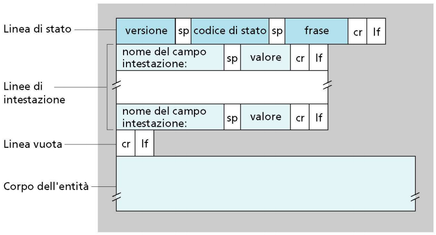
\includegraphics[scale=0.4]{Immagini/Http_res.png}
		\caption{In figura un messaggio di risposta.}
	\end{minipage}
\end{figure}
\newpage
\begin{figure}[!h]
	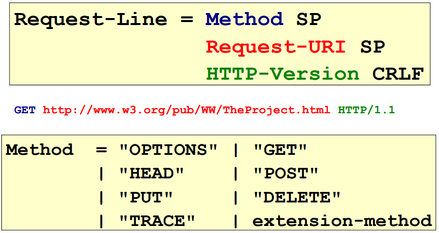
\includegraphics[scale=0.3]{Immagini/Req_line.png}
	\centering
	\caption{La struttura della \textbf{request line}. Il campo \textbf{method} è case sensitive ed indica l'operazione da eseguire sulla risorsa identificata dalla URI. Il metodo \textbf{POST} serve per inviare dal client al server le
		informazioni inserite nel body del messaggio, \textbf{PUT} è usato dal client per chiedere al server di creare o modificare una risorsa, \textbf{DELETE} per cancellarla.}
\end{figure}
\begin{figure}[!h]
	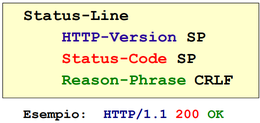
\includegraphics[scale=0.4]{Immagini/Stat_line.png}
	\centering
	\caption{La \textbf{status-Line} è la prima riga del messaggio di risposta. Lo \textbf{status code} è un numero di 3 cifre, indica il risultato del tentativo di soddisfare la richiesta del client. La \textbf{reason-phrase} dà una breve descrizione testuale dello status-code. Lo status-code è rivolto alla macchina mentre la reason-phrase all'utente umano.}
\end{figure}
Gli \textbf{header} sono insiemi di coppie \textbf{nome} : \textbf{valore} che specificano
alcuni parametri del messaggio trasmesso o ricevuto.
\begin{itemize}
	\item \textbf{General Headers}: sono relativi alla \textbf{trasmissione} e si applicano a \textbf{tutto il messaggio}. \textit{(e.g. \textbf{Date, Connection:} usato dal mittente per specificare delle opzioni desiderate per la connessione, ad esempio \underline{close}. \textbf{Transfer-encoding}: specifica se e quali trasformazioni sono state applicate al corpo del messaggio ad esempio gzip, chunked ecc. \textbf{Cache control}: indica quale tipologia di cache può memorizzare il messaggio, può essere \textbf{public}, \textbf{private} o \textbf{no-cache}.)}
	\item \textbf{Entity Headers}: sono \textbf{metadati} relativi all'\textbf{entità trasmessa}. Ogni entity è costituita da un \textbf{entity body} e da una
	      serie di \textbf{entity headers} che ne definiscono contenuto e
	      proprietà. \textit{(e.g. Content Lenght)}
	\item \textbf{Request Headers}: sono relativi alla \textbf{richiesta}. Supportano il \textbf{content negotiation}, il processo tramite cui il server sceglie la forma "giusta" del contenuto richiesto dal client. \textit{(Specificano da chi è fatta la richiesta, a chi viene fatta, che tipo di risposte il client è in grado di accettare, l'autorizzazione, ecc.)}
	\item \textbf{Response Headers}: sono relativi al \textbf{messaggio di risposta}.
\end{itemize}
\newpage
\begin{figure}[!h]
	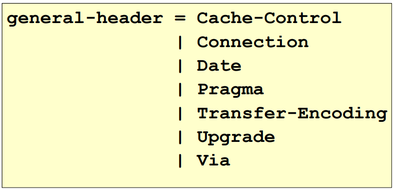
\includegraphics[scale=0.31]{Immagini/General_h.png}
	\centering
	\caption{L'elenco dei general headers.}
\end{figure}
\begin{figure}[!h]
	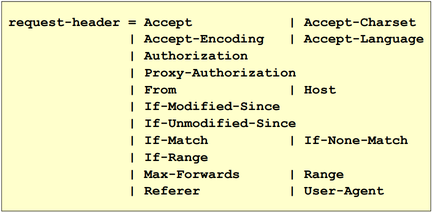
\includegraphics[scale=0.3]{Immagini/Req_h.png}
	\centering
	\caption{L'elenco dei request headers. \textbf{Accept} specifica quali tipi di media sono accettati in risposta dal client, \textbf{Accept-Charset}, quali caratteri e \textbf{Accept-Encoding} quali formati.}
\end{figure}
\begin{figure}[!h]
	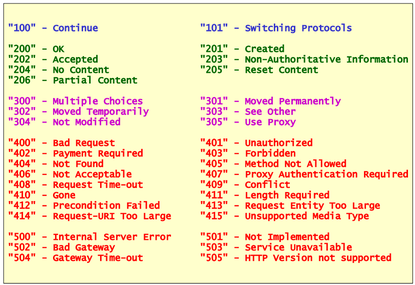
\includegraphics[scale=0.34]{Immagini/Stat_code.png}
	\centering
	\caption{In figura l'elenco degli status-codes e il loro significato.}
\end{figure}
\begin{figure}[!h]
	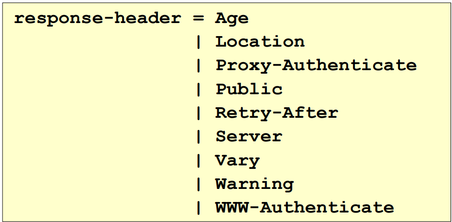
\includegraphics[scale=0.3]{Immagini/Resp_h.png}
	\centering
	\caption{I campi del \textbf{response-header} consentono al server di inviare informazioni aggiuntive che non possono essere poste nella status-line. Ad esempio: \textbf{Age}: indica quanto tempo è trascorso, in secondi, tra l'invio della risposta da parte del mittente e la generazione della stessa all'origine. \textbf{Location} é usato per reindirizzare il client verso un altra URI per completare la sua richiesta o per fornire una nuova risorsa. Il campo \textbf{Server} contiene informazioni sul software usato dal server di origine per portare a compimento la richiesta del client.}
\end{figure}
\newpage
Fin'ora abbiamo mostrato come il client accede alle risorse del web inviando richieste al server. Cosa succederebbe se, ad esempio, un client richiedesse continuamente la \textbf{stessa} risorsa? Potremmo evitare di inoltrare richieste tutte uguali al server?\newline
\textbf{Sì}, ci viene in aiuto il \textbf{web caching}. L'obbiettivo del web caching è di soddisfare le richieste del client \textbf{senza} contattare il server. Funziona memorizzando \textbf{copie temporanee} di risorse web, servendole poi al client così da \textbf{ridurre} l’uso di \textbf{banda}, limitare il \textbf{workload} sul server e di conseguenza \textbf{diminuire tempo di risposta} verso gli altri clients.\newline
Consideriamo due modelli possibili di web caching:
\begin{itemize}
	\item \textbf{User Agent Cache}: lo \textbf{user agent} (il browser) mantiene una \textbf{copia} delle risorse visitate dall’utente.
	\item \textbf{Proxy Cache}: il \textbf{proxy intercetta il traffico} e mette in cache le risposte. Successive richieste alla stessa URI possono essere servite direttamente dal proxy senza inoltrare la richiesta al server. Sta poi all' utente configurare il browser per consentire gli accessi Web via proxy.
\end{itemize}

\textit{Cos'è un proxy?}
\theoremstyle{definition}
\begin{definition}
	Un \textbf{proxy} è un \textbf{programma intermediario} che agisce sia da \textbf{server} che da \textbf{client}, \textbf{inviando} e \textbf{servendo} \textbf{richieste} per altri clients. Le richieste sono gestite internamente oppure sono girate a server terzi.
\end{definition}
Resta ora da chiarire come è possibile che, sebbene abbiamo definito il protocollo HTTP come \textbf{stateless}, alcuni siti, \textit{riconoscano} gli utenti.\newline
Sebbene infatti il protocollo HTTP sia a tutti gli effetti stateless, le applicazioni web \textbf{non} lo sono. Come fare quindi a conciliare queste due realtà?\newline\newline
\textit{Con i cookies!}
\begin{definition}
	I \textbf{cookies} sono stringhe di testo contenenti informazioni relative all'utente.
\end{definition}
I \textbf{cookies} funzionano nel seguente modo:
\begin{enumerate}
	\item Un client invia al server una richiesta HTTP.
	\item Il server invia al client la risposta HTTP e in più una linea \textbf{set-cookie: 1678453}. \textit{(esempio fittizio)}
	\item Il client \textbf{memorizza} il cookie in un file e lo associa al server.
	      Lo aggiungerà con la seguente linea: \textbf{cookie: 1678453} a tutte le sue successive richieste.
	\item Alla successiva richiesta da parte del client, il server \textbf{risalirà} tramite il cookie alle informazioni ad esso \textbf{associate}.
\end{enumerate}
\newpage

\subsubsection{TELNET}
\textbf{TELNET}, acronimo per \textbf{TE}rmina\textbf{L} \textbf{NET}work, è un \textbf{protocollo} \textbf{client-server} che fornisce una comunicazione \textbf{interattiva ed orientata al testo} tra due macchine, è basato sul trasporto \textbf{connection-oriented} ed usa il protocollo \textbf{TCP}.
Consente all'utente di effettuare una sessione di \textbf{login} in una macchina remota e quindi di utilizzarne il terminale. L'utente che si autentica tramite login remoto ha accesso infatti a tutti i \textbf{comandi} e ai \textbf{programmi} disponibili su di essa. \textbf{I comandi vengono eseguiti come se l'utente li digitasse dalla tastiera stessa della macchina.} \textit{Per estensione,} \texttt{\textbf{telnet}} \textit{è anche il nome di un programma usato per avviare una sessione TELNET verso un host remoto.}
\textbf{TELNET} infatti include due programmi: un programma \textbf{TELNET client} e un programma \textbf{TELNET server}. \textbf{TELNET client} (\texttt{\textbf{telnet}}) interagisce con l'utente sulla macchina locale e scambia messaggi con \textbf{TELNET server}. Riportiamo di seguito una semplificazione del funzionamento:
\begin{enumerate}
	\item L'utente, dalla \textbf{propria} macchina \textbf{locale} (\textbf{\textbf{TELNET client}}), stabilisce una connessione \textbf{TCP}, persistente per tutta la durata della sessione, con una \textbf{macchina remota (\textbf{TELNET server})} alla \textbf{porta 23} e vi si \textbf{autentifica}.
	\item  Tutte le \textbf{battute} dei \textbf{tasti} della macchina locale vengono \textbf{trasmesse} dal client
	      alla \textbf{macchina remota}.
	\item La \textbf{macchina remota} accetta la connessione TCP e il \textbf{TELNET server} trasmette i dati al sistema operativo locale.
	\item L'\textbf{output} della \textbf{macchina remota} viene quindi \textbf{ricevuto} e \textbf{trasmesso} sul terminale dell'utente.
\end{enumerate}
\begin{figure}[!h]
	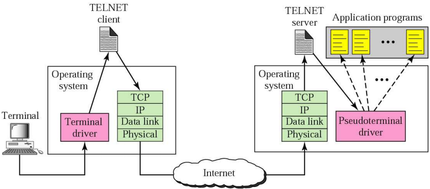
\includegraphics[scale=0.8]{Immagini/TELNET.png}
	\centering
	\caption{In figura il funzionamento di TELNET.}
\end{figure}
\underline{N.B. TELNET è un protocollo STATEFUL.}
\newpage
\textit{Problema: come operare con sistemi operativi diversi?}\newline\newline
I terminali infatti non sono tutti uguali, possono differire gli uni dagli altri per il \textbf{set} e la \textbf{codifica} dei caratteri, per la \textbf{lunghezza} della \textbf{linea} e della \textbf{pagina} e per i \textbf{tasti funzione} individuati da diverse sequenze di caratteri. \newline\newline
Una \textbf{soluzione} è stata trovata mediante la definizione di un \textbf{Network Virtual  Terminal (NVT) che definisce un \textbf{set di caratteri universali}}.
L’NVT è quindi un dispositivo “immaginario” che fornisce una
rappresentazione astratta di un terminale. Gli host, sia client
che server, \textbf{traducono} le loro caratteristiche \textbf{locali} \textbf{tramite il set universale} così da apparire \textbf{in rete} come un NVT e assumono che l’host remoto sia anch'esso un NVT. Questa operazione di traduzione è ovviamente \textbf{reversibile}.
\begin{figure}[!h]
	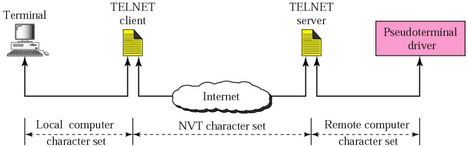
\includegraphics[scale=0.6]{Immagini/NVT.png}
	\centering
\end{figure}
\newline
Il funzionamento di TELNET, con l'aggiunta della trasformazioni intermedie sopra descritte diventa:
\begin{enumerate}
	\item ...
	\item  Tutte le \textbf{battute} dei \textbf{tasti} della macchina locale vengono \textbf{trasformate in NVT e successivamente} \textbf{trasmesse dal TELNET client}
	      alla \textbf{macchina remota}.
	\item La \textbf{macchina remota} accetta la connessione TCP, il \textbf{TELNET server} \textbf{traduce} da NVT allo standard del sistema operativo remoto e infine gli trasmette i dati ricevuti.
	\item ...
\end{enumerate}
\begin{figure}[!h]
	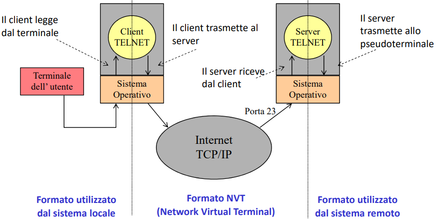
\includegraphics[scale=0.5]{Immagini/NVT2.png}
	\centering
\end{figure}
\underline{\textit{N.B. NVT invia i caratteri di controllo prioritariamente con TCP URGENT.}}
\newpage
Concludiamo con qualche tecnicismo: \newline\newline
I terminali NVT si scambiano dati in formato \textbf{7-bit US-ASCII} e adottano inoltre un approccio \textbf{in-band signaling}, ovvero dati e comandi viaggiano sullo \textbf{stesso canale}. Per distinguere i due tipi di informazione si usa la seguente convenzione: ogni carattere è inviato come un \textbf{ottetto di bit} con \textbf{il primo bit settato a zero}. I caratteri, in notazione decimale, vanno dal numero 0 al 127. I comandi invece sono identificati tramite  ottetti speciali di 1, in n. d. vanno dal numero 240 al numero 254, per distinguerli dai dati sono sempre preceduti da un carattere speciale: \textbf{IAC o Interpret As Command} identificato, sempre in n. d., dal numero 255. Essenzialmente quindi si usa un canale di 8 bit per scambiare dati di tipo 7 bit ASCII. I messaggi scambiati durante la fase iniziale della comunicazione, ovvero prima del login, sono \textbf{messaggi di controllo} e costituiscono la \textbf{Telnet Option Negotiation}, in sostanza sono usati per scambiare \textbf{informazioni} sulle \textbf{caratteristiche} degli \textbf{host}.
\begin{table}[h!]
	\begin{center}
		\label{tab:table1}
		\begin{tabular}{l|c|r}
			\textbf{Comando} & \textbf{Codifica decimale} & \textbf{Significato} \\
			\hline
			IAC              & 255                        & Interpret as command \\
			EL               & 248                        & Erase line           \\
			EC               & 247                        & Erase character      \\
			IP               & 244                        & Interrupt process    \\
			EOR              & 239                        & End of record        \\
		\end{tabular}
	\end{center}
\end{table}\newline
\textit{Ma quindi NVT conviene?}\newline\newline
Rispondiamo alla domanda mostrando dei semplici calcoli:\newline\newline
Supponiamo che N sia il numero di sistemi distinti che si vogliono far
interoperare:
\begin{itemize}
	\item \textbf{Senza} l'uso di NVT, si necessita la scrittura di \textbf{N-1} client per ogni sistema (N-1 TELNET-clients che traducano negli N-1 standards dei sistemi), e 1 TELNET-server per ogni sistema: \newline
	      In totale si avranno $N\times(N-1) + N$ applicativi.
	\item \textbf{Usando} NVT, bisogna scrivere 1 TELNET-server per ogni sistema e N TELNET-client (1 per ogni sistema che traduca dallo standard di sistema allo standard di NVT): \newline Avremo quindi $N + N = 2N$ applicativi.
\end{itemize}
Quindi per $N > 2$ \textbf{conviene} usare NVT!
\newpage
\subsubsection{SSH}
TELNET non possiede \textbf{alcuna} misura di sicurezza poichè è stato progettato per l'uso su \textbf{reti private}, trasmette tutto in chiaro, anche le \textbf{password}! Con l'avvento delle reti pubbliche però si è reso necessario prendere delle contromisure. \newline
\textbf{SSH} o \textbf{S}ecure \textbf{SH}ell è un'applicazione nata per sostituire TELNET.
\begin{figure}[!h]
	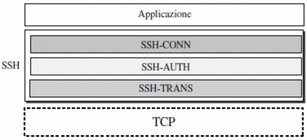
\includegraphics[scale=0.7]{Immagini/SSH.png}
	\centering
	\caption{Le componenti di SSH}
\end{figure}\newline
Il \textbf{protocollo} di livello applicazione \textbf{SSH} è composto da \textbf{tre} diverse componenti: \textbf{SSH-TRANS, SSH-AUTH e SSH-CON}. La componente \textbf{SSH-TRANS} o \textbf{SSH-Transport Layer Protocol} costruisce un canale di comunicazione sicuro, tramite tecniche crittografiche, sfruttando la connessione offerta da TCP. Il \textbf{protocollo TCP} trasmette tutte le informazioni in chiaro, \textbf{non} è quindi in grado \textbf{da solo} di garantire \textbf{privacy} e \textbf{confidenza}. \textit{SSH-TRANS è anche in grado di riconoscere se il server a cui ci stiamo connettendo è quello autentico o meno.} La componente \textbf{SSH-AUTH} si occupa di autenticare il client. \textit{Sono disponibili altre tecniche di autenticazione oltre alla classica con username e password tra le quali l'accesso basato su coppie di chiavi crittografiche.} Infine la componente \textbf{SSH-CONN} sfruttando i servizi offerti dalle altre due componenti offre i servizi di \textbf{terminale}, \textbf{trasferimento file}, \textbf{creazione di tunnel} ecc...\newline \textbf{SSH offre} quindi \textbf{molti più servizi di TELNET}.\newline\newline
\textit{Cos'è il TCP Port Forwarding?}\newline\newline
Il \textbf{TCP Port Forwarding} è un meccanismo che permette di \textbf{creare} un \textbf{canale di comunicazione sicuro} attraverso il quale \textbf{veicolare} \textbf{qualsiasi} tipo di \textbf{connessione TCP}. Opera creando un canale di comunicazione \textbf{cifrato} tra la \textbf{porta} all’\textbf{indirizzo remoto} a cui ci si vuole collegare e una \textbf{porta locale} libera. Le applicazioni punteranno il collegamento alla porta locale e la connessione verrà inoltrata automaticamente all’host remoto
tramite un canale sicuro. \newline Segue una spiegazione delle differenze tra \textbf{local port forwarding} e \textbf{remote port forwarding}.
\newpage
\begin{itemize}
	\item \textbf{Local}: \texttt{ssh -L} specifica che il traffico sulla porta indicata della macchina locale deve essere reindirizzato verso la porta indicata della macchina remota. \newline
	      e.g. \texttt{ssh -L sourcePort:forwardToHost:onPort connectToHost} significa: connettiti via ssh a \textbf{connectToHost}, e inoltra tutti i tentativi di connessione che arrivano alla porta locale \textbf{sourcePort} verso la porta \textbf{onPort} della macchina chiamata \textbf{forwardToHost}, che si raggiunge tramite la macchina chiamata a sua volta \textbf{connectToHost}.
	      \begin{figure}[!h]
		      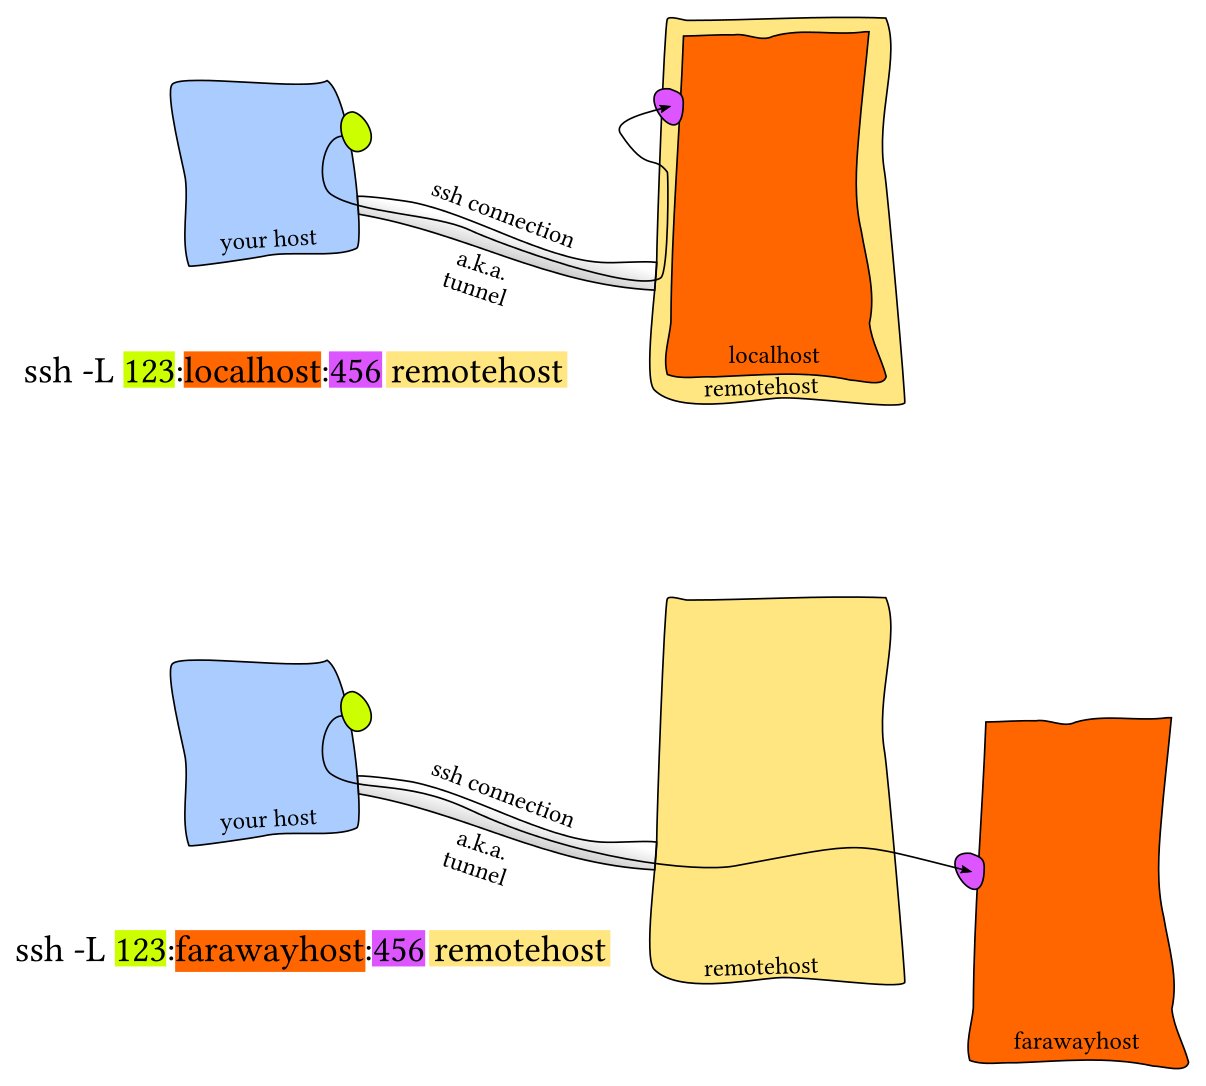
\includegraphics[scale=0.8]{Immagini/Local_ssh.png}
		      \centering
	      \end{figure}
	      \newpage
	\item \textbf{Remote}: \texttt{ssh -R} specifica che il traffico sulla porta indicata della macchina remota deve essere reindirizzato verso la porta indicata della macchina locale.\newline
	      e.g. \texttt{ssh -R sourcePort:forwardToHost:onPort connectToHost} significa: connettiti via ssh a \textbf{connectToHost}, e inoltra tutti i tentativi di connessione che arrivanao alla porta remota \textbf{sourcePort} verso la porta \textbf{onPort} della macchina \textbf{forwardToHost}, che si raggiunge tramite la tua macchina locale.
	      \begin{figure}[!h]
		      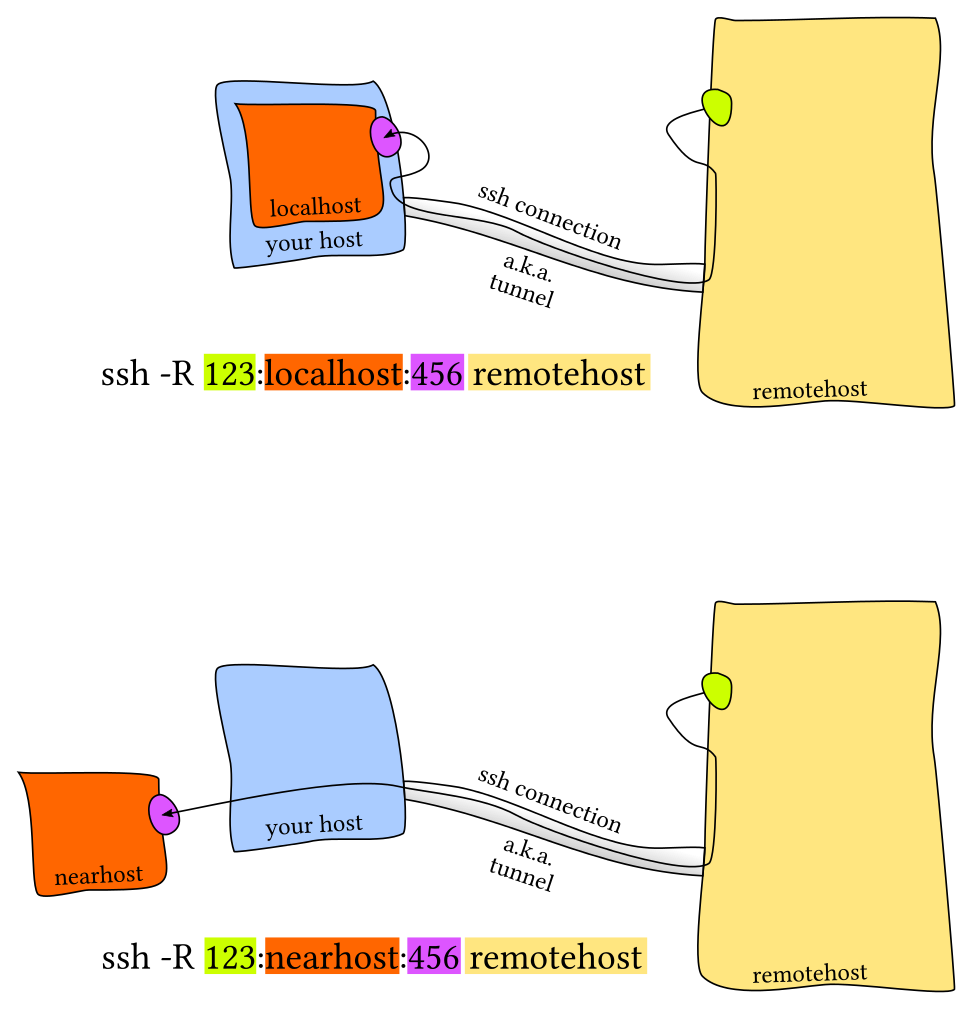
\includegraphics[scale=0.9]{Immagini/Remote_ssh.png}
		      \centering
	      \end{figure}
\end{itemize}
\underline{N.B. SSH è un protocollo STATEFUL.}
\newpage
\subsubsection{FTP}
\label{sec:FTP}
\textbf{FTP} acronimo per \textbf{F}ile \textbf{T}ransfer \textbf{P}rotocol, è un \textbf{protocollo} per il \textbf{trasferimento} di \textbf{dati} tra due host di una rete, è lo \textbf{standard} per il \textbf{trasferimento} di file \textbf{offerto da TCP/IP}. Adotta il modello \textbf{client-server}: il \textbf{client} richiede il trasferimento di un file che può consistere sia nell'\textbf{acquisizione} di una copia locale modificabile sia nell'eventuale \textbf{trasferimento} della copia modificata sull'host remoto (\textbf{server}).
\begin{figure}[!h]
	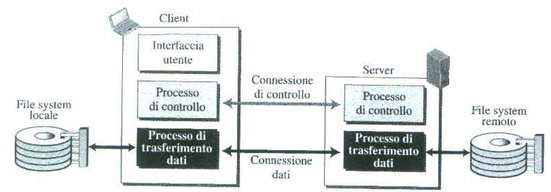
\includegraphics[scale=0.4]{Immagini/FTP.png}
	\centering
\end{figure}\newline
Il \textbf{client} ha \textbf{tre} componenti: \textbf{interfaccia utente}, \textbf{processo di controllo} e \textbf{processo di trasferimento dati} mentre il \textbf{server} remoto ne ha solo \textbf{due}: \textbf{processo di controllo} e \textbf{processo di trasferimento dati}. La \textbf{separazione} del trasferimento dei dati da quello dei comandi rende il protocollo FTP \textbf{efficiente}. Infatti la \textbf{connessione di controllo} usa \textbf{regole semplici} così da ridurre lo scambio delle informazioni a \textbf{una riga di comando} e \textbf{una di risposta per ogni interazione}. Mentre la \textbf{connessione dati usa regole più complicate} a causa della varietà delle informazioni che vi transitano.
\textbf{FTP} offre funzionalità \textbf{aggiuntive} oltre al semplice trasferimento di dati, infatti \textbf{mette a disposizione}:
\begin{itemize}
	\item \textbf{Accesso interattivo}: l’utente può \textbf{navigare}, \textbf{cambiare} e \textbf{modificare} l’albero di directory nel file system dell'host remoto.
	\item \textbf{Specificazione del formato dei dati da trasferire} (e.g. file di testo o file binari)
	\item \textbf{Autenticazione}: il client può \textbf{autenticarsi} con username e password.
\end{itemize}
Poco sopra abbiamo accennato al fatto che \textbf{FTP} prevede l'instaurazione di \textbf{due tipi di connessione tra il client e il server} ovvero:
\begin{enumerate}
	\item \textbf{Control connection}: prevede uno scambio di comandi e risposte
	      tra client e server. Segue il protocollo TELNET e \textbf{rimane aperta per l'intera durata della sessione interattiva}. Si usa la \textbf{porta 21} del \textbf{server} e la codifica standard \textbf{NVT ASCII}.
	\item \textbf{Data connection}: prevede il trasferimento di dati mediante procedure e la \textbf{specifica dei tipi}. I dati trasferiti possono essere parte di un file, un file o un set di file. \textbf{Viene aperta e chiusa per ogni singolo scambio}. Per lo scambio di dati il \textbf{server} usa la \textbf{porta 20}.
\end{enumerate}
\newpage
La \textbf{Data Connection} \textbf{non segue il protocollo TELNET} e la sua apertura avviene secondo uno schema completamente diverso, ovvero:
\begin{enumerate}
	\item Il \textbf{client}, non il server, effettua un'\textbf{apertura} \textbf{passiva} usando una \textbf{porta effimera} e resta in attesa di connessione, viene fatto dal client poichè è tale processo che invierà i comandi, tramite la connessione di controllo, per il trasferimento dei file.
	\item Il client \textbf{invia} questo \textbf{numero} di \textbf{porta} al \textbf{server} per mezzo del comando PORT.
	\item Il \textbf{server}, ricevuto il numero di porta, \textbf{effettua} un'\textbf{apertura} \textbf{attiva}, ovvero apre la connessione, usando la propria \textbf{porta} nota \textbf{20} e quella effimera offerta dal client.
\end{enumerate}
Per effettuare il trasferimento dei file inoltre, il client deve \textbf{definire} il \textbf{tipo}
di file, la \textbf{struttura dati} e la \textbf{modalità di trasmissione} al fine di
risolvere i problemi di eterogeneità tra client e server, va infatti ricordato che programma client e programma server sono su macchine \textbf{diverse}. Questo scambio di informazioni avviene mediante la \textbf{connessione di controllo}.\newline\newline
FTP è quindi un protocollo \textbf{STATEFUL} poichè il \textbf{server deve tener traccia dello stato dell’utente}: bisogna tenere conto infatti, tra le altre cose, della directory del file system remoto in cui si trova l'utente!\newline\newline
Concludiamo menzionando il fatto che esistono server che supportano connessioni FTP \textbf{senza autenticazione} (\textbf{Anonymous FTP}).  Tipicamente consentono di accedere \textbf{solo} ad una parte del file system e permettono \textbf{solo} un subset di operazioni (e.g. la PUT \textbf{non} è permessa). Di solito \textbf{si usa} un \textbf{username comune} (solitamente "ftp" or "anonymous") e una \textbf{password qualsiasi} (e.g. l'indirizzo email dell'utente).\textit{ Erano usate per distribuire a un pubblico dei file senza dover generare numerosi username e password.}
\begin{table}[h!]
	\begin{center}
		\label{tab:table1}
		\begin{tabular}{l|c|r}
			\textbf{Comandi di controllo} & \textbf{Significato}             \\
			\hline
			USER                          & username                         \\
			PASS                          & password                         \\
			LIST                          & elenca i file della
			directory corrente                                               \\
			NLST                          & richiede elenco file e
			directory (ls)                                                   \\
			RETR filename                 & recupera (get)
			un file dalla directory
			corrente                                                         \\
			STOR filename                 & memorizza
			(put) un file nell’host remoto                                   \\
			ABOR                          & interrompe l’ultimo
			comando ed i trasferimenti in
			corso                                                            \\
			PORT                          & indirizzo e numero di porta
			del client                                                       \\
			SYST                          & il server restituisce il tipo di
			sistema                                                          \\
			QUIT                          & (quit) chiude la
			connessione                                                      \\
		\end{tabular}
	\end{center}
\end{table}
\newpage
\subsubsection{DNS}
Sappiamo oramai che i dispositivi connessi in rete vengono individuati dai protocolli TCP/IP mediante i loro \textbf{indirizzi IP}, gli utenti, d'altro canto, preferiscono usare dei \textbf{nomi} invece che degli indirizzi numerici. Un \textbf{nome} identifica un \textbf{oggetto} mentre un \textbf{indirizzo} specifica \textbf{dove} l'oggetto è situato.\newline\newline
\textit{Come fare per associare i nomi agli indirizzi?}\newline\newline
Agli albori di Internet l’associazione tra nomi logici e indirizzi IP era statica!
Tutti i nomi \textit{logici} e i relativi indirizzi IP erano contenuti in un file chiamato \textbf{host file} e periodicamente tutti gli host ne prelevavano una versione aggiornata, chiamata a sua volta \textbf{master host file}, da un server ufficiale.\newline
A noi utenti moderni però dovrebbe immediatamente saltare all'occhio la seguente \textbf{problematica}: le \textbf{dimensioni attuali di Internet} rendono questo approccio \textbf{impraticabile}. Non sarebbe infatti possibile che ogni host possegga una \textbf{copia aggiornata} di un elenco del genere, in più la dimensione di questo  sarebbe sterminata, per non parlare del \textbf{volume di traffico} sul server ufficiale, il pericolo dovuto alla presenza di un \textbf{unico punto di fallimento} e l'\textbf{impossibilità di scalare} di questo sistema.\newline
Fu così che all'inizio degli anni '80 venne ideato il \textbf{DNS} o \textbf{Domain Name System}. L'\textbf{idea centrale} è di \textbf{suddividere} la sconfinata mole di associazioni nome-indirizzo e \textbf{distribuirne} le varie parti su \textbf{calcolatori sparsi per il mondo}. \textit{Come funziona? Così:}
\begin{figure}[!h]
	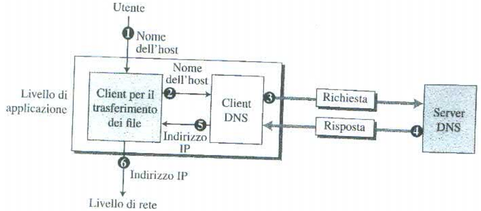
\includegraphics[scale=0.8]{Immagini/DNS.png}
	\centering
\end{figure}\newline
Supponiamo che un utente utilizzi un client di trasferimento file per accedere a un file su un server. L'utente conoscerà solo il \textbf{nome} del server e.g. \textit{cheneso.com}, lo \textbf{stack TCP/IP} invece ha bisogno dell'\textbf{indirizzo IP} del server per stabilire una connessione. Alla pagina seguente troviamo i sei passi necessari per \textbf{associare} l'\textbf{indirizzo} IP al \textbf{nome} del server.
\newpage
\begin{enumerate}
	\item L'\textbf{utente} comunica il nome del server al client di trasferimento file.
	\item \textbf{Il client di trasferimento file} trasmette il nome del server al \textbf{client DNS}.
	\item \textbf{Ogni computer una volta avviato conosce l'indirizzo IP di un server DNS}, il \textbf{client DNS} invia dunque, usando la \textbf{porta 53}, al \textbf{server DNS} la richiesta di traduzione del nome simbolico del server.
	\item Il \textbf{server DNS} risponde con l'indirizzo IP del server desiderato.
	\item Il \textbf{client DNS} comunica al \textbf{client di trasferimento file} l'indirizzo IP del server.
	\item Il \textbf{client di trasferimento file} \textbf{utilizza} così l'\textbf{indirizzo IP ricevuto} per accedere al server.
\end{enumerate}
Per far sì che questo meccanismo funzioni bisogna \textbf{eliminare le ambiguità sui nomi} e per far ciò si è definito uno \textbf{spazio dei nomi}. Lo \textbf{spazio dei nomi} ha una \textbf{struttura gerarchica} per una ragione principale: se tutti i nomi fossero composti da una sola stringa alfanumerica servirebbe un'\textbf{autorità centrale} che controllasse l'unicità di ogni singolo nome. Una \textbf{struttura gerarchica} consente invece di avere nomi composti da diverse parti e di \textbf{delegare il controllo} su ciascuna parte a enti o società diverse, \textbf{decentralizzando} in tal modo il processo di controllo.
\begin{figure}[!h]
	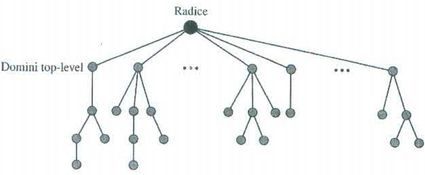
\includegraphics[scale=0.7]{Immagini/DNSpace.png}
	\centering
	\caption{In figura lo spazio dei nomi di dominio.}
\end{figure}\newline
Nello \textbf{spazio dei nomi di dominio} i nomi hanno una struttura ad \textbf{albero} con la radice in cima e un numero di livelli compreso tra 0 e 127. Ogni nodo è individuato da un'\textbf{etichetta} costituita da \textbf{massimo 63 caratteri} (\textit{la radice ha l'etichetta vuota}), tutti i nodi collegati a uno stesso nodo da rami diversi hanno etichette \textbf{diverse}, ciò garantisce l'\textbf{univocità} dei nomi. Ogni nodo dell'albero ha inoltre un \textbf{nome di dominio}, che, se letto da sinistra verso destra, è costituito da tutte le etichette, separate da punti, di tutti i nodi a partire dal nodo stesso fino alla radice, la cui etichetta è la stringa \textbf{nulla}. Immediatamente sotto la radice si trovano i \textbf{domini top-level}.
\newpage
\begin{figure}[!h]
	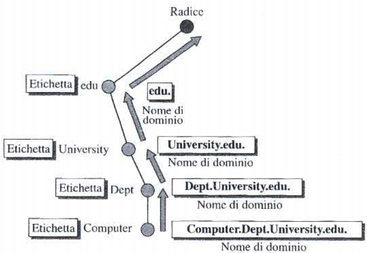
\includegraphics[scale=0.7]{Immagini/Etichette_dns.png}
	\centering
	\caption{In figura le etichette e i nomi di dominio.}
\end{figure}
\theoremstyle{definition}
\begin{definition}
	Un \textbf{dominio} è un \textbf{sottoalbero} dello spazio dei nomi che viene identificato dal \textbf{nome di dominio} della sua radice.
\end{definition}
\textit{Ma dove sono contenute le informazioni relative allo spazio dei nomi di dominio?}

\begin{figure}[!h]
	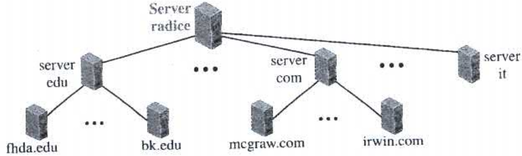
\includegraphics[scale=0.6]{Immagini/Dnserver.png}
	\centering
	\caption{In figura la gerarchia dei name server.}
\end{figure}
All'interno dei \textbf{DNS-Servers} o \textbf{name servers}. L'intero spazio dei nomi è stato \textbf{diviso} in diversi domini, differenziati al \textbf{top-level}, e i domini così ottenuti sono stati divisi a loro volta ottenendo dei sotto domini. Ogni \textbf{name server} è responsabile di un dominio o di un sottodominio. Vi è quindi una \textbf{gerarchia di server}. Una \textbf{zona} \textbf{è tutto ciò di cui è responsabile un server}, se un server è responsabile di un dominio e non effettua suddivisioni in sottodomini, allora la sua zona e il suo dominio \textbf{coincidono}. Se invece il server suddivide il proprio dominio in sottodomini la sua zona e il suo dominio \textbf{differiscono}. Ogni name-server ha un database chiamato \textbf{file di zona} contenente le informazioni su tutti i nodi che ricadono nella \textbf{sua} \textbf{zona} di competenza. \newpage Un \textbf{root server} è un server che ha per zona l'\textbf{intero albero dello spazio dei nomi}.\newline Solitamente i \textbf{root server} si limitano a immagazzinare riferimenti relativi ad altri server e \textbf{delegano} loro tutte le responsabilità.\newline
Esempio di top-level domains:
\begin{table}[h!]
	\begin{center}
		\label{tab:table1}
		\begin{tabular}{l|c|r}
			\textbf{Dominio}     & \textbf{Uso}                            \\
			\hline
			com                  & organizzazioni commerciali              \\
			edu                  & istituti di istruzione                  \\
			mil                  & gruppi militari                         \\
			gov                  & istituzioni governative americane       \\
			net                  & principali centri di supporto alla rete \\
			org                  & organizzazioni diverse dalle precedenti \\
			it, uk, us, fr, ecc. & codice geografico per nazioni
			\\
		\end{tabular}
	\end{center}
\end{table}\newline
I \textbf{server DNS} possono essere \textbf{primari} o \textbf{secondari}.
\begin{itemize}
	\item Un server \textbf{primario} possiede sul disco e aggiorna il \textbf{file di zona} relativo alla zona sotto la sua responsabilità.
	\item Un server \textbf{secondario} riceve le informazioni relative a una zona da un \textbf{server primario}.
\end{itemize}
I \textbf{server} \textbf{primari} e \textbf{secondari} hanno la medesima autorità sulla loro zona di competenza, è bene specificare che \textbf{un server può essere primario per una zona  e secondario per un altra}, \textbf{primario} e \textbf{secondario} sono quindi aggettivi \textbf{relativi alla zona}. Si noti inoltre come l'introduzione di un server secondario in una zona porti a una duplicazione del \textbf{file di zona} che può risultare utile per eventuali guasti al \textbf{server primario}.\newline\newline
\textit{Come si associa l'indirizzo IP da un nome?}\newline\newline
Il processo con cui si associa l'indirizzo IP da un nome è detto \textbf{processo di risoluzione}. Il \textbf{protocollo DNS} è progettato come protocollo \textbf{client-server}. Un host che voglia ricavare un indirizzo IP da un nome si rivolge al \textbf{programma client} detto anche \textbf{resolver} che invierà un'opportuna richiesta al \textbf{server DNS più vicino} il quale, se dispone della risposta, invierà l'indirizzo o il nome (\textit{è infatti possibile fare il processo al contrario}), oppure inoltrerà la richiesta a un altro server o comunicherà al resolver l'indirizzo di un altro server a cui fare riferimento. Il \textbf{resolver}, ricevuta la risposta, la esaminerà per verificarne la presenza di errori e la trasmetterà al processo che l'ha effettuata. La \textbf{risoluzione} può essere \textbf{ricorsiva} o \textbf{iterativa}.
\newpage

\begin{itemize}
	\item Con la \textbf{risoluzione ricorsiva}, la \textbf{query DNS} viaggia dall'host su cui è in esecuzione il processo applicativo che ne ha fatto richiesta fino a un host che conosce l'indirizzo IP richiesto, eventualmente scalando, poi discendendo e infine percorrendo a all'indietro \textbf{l'intera gerarchia dei server DNS}. \textbf{Al server locale che ha richiesto la query viene inviato \textbf{solo} l'indirizzo IP risultante}, ha richiesto quindi una \textbf{conversione completa}.
	      \begin{figure}[!h]
		      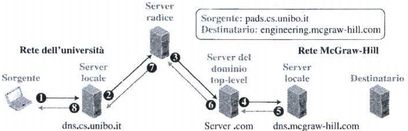
\includegraphics[scale=0.7]{Immagini/DNSrec.png}
		      \centering
		      \caption{In figura un esempio di risoluzione ricorsiva.}
	      \end{figure}
	\item Con la  \textbf{risoluzione iterativa} ogni \textbf{server-DNS} che non è in grado di risolvere la \textbf{query-DNS} dell'host risponde, \textbf{direttamente al server locale}, con \textbf{l'indirizzo di un altro server in grado di risolverla}.
	      \textbf{	Al server locale che ha richiesto la query non viene quindi inviato solo l'indirizzo IP risultante}. La \textbf{risoluzione iterativa} è supportata da \textbf{tutti} i \textbf{name server}, l'host può richiedere che venga usata la \textbf{risoluzione ricorsiva} ma potrebbe non essere disponibile.

	      \begin{figure}[!h]
		      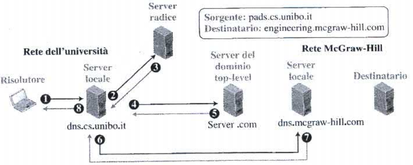
\includegraphics[scale=0.7]{Immagini/DNSite.png}
		      \centering
		      \caption{In figura un esempio di risoluzione iterativa.}
	      \end{figure}
\end{itemize}
Ogni volta che a un \textbf{server} arriva una richiesta di risoluzione di un nome, che non fa parte del suo dominio, deve cercare, all'interno del suo database, un altro server a cui inoltrare la richiesta. Ridurre questo tempo di ricerca significa ridurre il tempo di attesa della risposta e aumentare l'efficienza. Ancora una volta ci viene in aiuto il \textbf{caching}: una volta che un \textbf{server} ha appreso un' \textbf{associazione}, la inserisce in \textbf{cache}. Il server marca le risposte prese dalla propria cache come \textbf{unauthoritative} o non autorevole.
\newpage
Dopo un certo lasso di tempo chiamato \textbf{TTL} o \textbf{time to live} il server cancella dalla cache l'associazione per evitare l'invio di risposte obsolete.\newline\newline
\textit{Ma come è fatto quindi il database di un server?}\newline\newline
Il \textbf{database del server} non è altro che una collezione di \textbf{records} strutturati nel seguente modo:\newline\newline
\centerline{\textbf{(Nome di dominio, Tipo, Classe, TTL, Valore)}}\newline\newline
A ogni \textbf{nome di dominio}, quindi a ogni \textbf{nodo dell'albero dello spazio dei nomi di dominio}, è associato un record composto da 5 campi.
\begin{itemize}
	\item \textbf{Nome di dominio} identifica il record della risorsa.
	\item \textbf{Tipo} definisce come interpretare il campo \textbf{Valore}.
	\item \textbf{Classe} definisce il tipo di rete, IN sta per Internet.
	\item \textbf{TTL} indica il numero di secondi per cui l'informazione deve essere ritenuta valida
	\item \textbf{Valore} contiene l'informazione memorizzata relativa al \textbf{nome di dominio}.
\end{itemize}
Di seguito i \textbf{tipi} dei \textbf{record}:
\begin{table}[h!]
	\begin{center}
		\label{tab:table1}
		\begin{tabular}{l|c|r}
			\textbf{Tipo} & \textbf{Interpretazione}                           \\
			\hline
			A             & indirizzo Ipv4 a 32 bit                            \\
			NS            & identifica i server autoritativi di una zona       \\
			CNAME         & il nome di dominio è un alias per quello ufficiale \\
			SOA           & informazioni autoritative riguardanti una zona     \\
			MX            & server di posta del dominio
			corrente                                                           \\
			AAAA          & indirizzo Ipv6                                     \\
		\end{tabular}
	\end{center}
\end{table}\newline
\textit{Che protocollo di livello trasporto è usato?}\newline\newline
Il sistema DNS può usare \textbf{sia} il \textbf{il protocollo TCP} che l'\textbf{UDP}.
Il \textbf{protocollo UDP} viene usato \textbf{quando} la dimensione del messaggio di risposta è \textbf{inferiore} a\textbf{ 512 byte}, molto spesso infatti i \textbf{datagrammi utente UDP} non possono superare i 512 byte come dimensione massima. In caso contrario si usa il \textbf{protocollo TCP}.\newline\newline
\textit{Come si aggiungono nuovi domini al DNS?}\newline\newline Pagando i \textbf{registrar}, ovvero aziende commerciali accreditate dall'ICANN.\newpage
\textit{Come sono fatti i messaggi DNS?}\newline\newline
I \textbf{messaggi DNS} posso essere di \textbf{due tipi}: di \textbf{interrogazione} o di \textbf{risposta} e i due tipi hanno lo \textbf{stesso} formato.
\begin{figure}[!h]
	\includegraphics[scale=0.6]{Immagini/DNSmessage.png}
	\centering
	\caption{La struttura dei messaggi DNS, il messaggio interrogazione contiene solo la sezione richiesta mentre il messaggio di risposta contiene la sezione richiesta, la sezione risposta ed eventualmente le altre due.}
\end{figure}\newline
Descriviamo ora brevemente i vari campi situati prima dell'\textbf{intestazione} lunga \textbf{12 bytes}:
\begin{itemize}
	\item \textbf{Identificazione} è il campo usato dal \textbf{client} per associare la risposta all'interrogazione.
	\item Il campo \textbf{Flag} indica se si tratta di un messaggio di richiesta o di risposta e segnala inoltre la presenza di eventuali errori.
	\item I \textbf{quattro} campi successivi dell'\textbf{intestazione} specificano il numero di ciascun tipo di record presente nel messaggio.
\end{itemize}
Poi del \textbf{messaggio}:
\begin{itemize}
	\item La \textbf{sezione di richiesta} che è inclusa nell'interrogazione e poi ripetuta anche nel messaggio di risposta è \textbf{formata} da\textbf{ uno o più record di richiesta}.
	\item La \textbf{sezione di risposta} è presente \textbf{esclusivamente} nei messaggi di risposta consiste \textbf{in uno o più record di risorsa}
	\item La \textbf{sezione autoritativa} fornisce le informazioni di uno o più server autorevoli per l'interrogazione.
	\item La \textbf{sezione supplementare} contiene \textbf{informazioni aggiuntive} che potrebbero essere \textbf{utili} al \textbf{client DNS}.
\end{itemize}
\textit{In UNIX si può utilizzare il comando} \texttt{nslookup} \textit{per ottenere associazioni nome simbolico : indirizzo numerico.}
\newpage
\subsubsection{EMAIL - SMTP}
\label{sec:SMTP}
La \textbf{posta elettronica} è uno dei primi servizi applicativi di Internet, la sua nascita risale infatti al 1971, quando un tale Ray Tomlinson installò su ARPANET un sistema in grado di scambiare messaggi fra le varie università. La \textbf{posta elettronica} consente agli utenti di scambiarsi \textbf{messaggi}, sebbene si siano trattate \textbf{altre applicazioni} fornenti questo servizio e.g. \textbf{HTTP} e \textbf{TCP}, il funzionamento della posta elettronica è tale da distinguersi da queste due applicazioni citate poco prima. Infatti in applicazioni come \textbf{FTP} e \textbf{HTTP} il programma \textbf{server} è \textbf{sempre attivo} e in attesa di richieste, che quando arrivano, vengono processate.
Vi è quindi una richiesta e una risposta. Nella \textbf{posta elettronica} il \textbf{funzionamento} è \textbf{differente}: infatti l'invio di un messaggio è considerato una \textbf{transazione unidirezionale}, la risposta può anche non arrivare e se arriva è considerata un'altra transazione unidirezionale. Secondariamente \textbf{non avrebbe} molto \textbf{senso tenere in esecuzione continuata un programma server} in attesa che qualcuno ci invii un messaggio, potremmo ragionevolmente voler spegnere il computer nell'attesa. Ciò implica che l'idea di modello client-server debba essere realizzata in un altro modo, magari utilizzando dei \textbf{server intermedi} e \textbf{disaccoppiando} le funzionalità di \textbf{ricezione} da quelle di \textbf{invio}. Di seguito illustriamo concisamente l'architettura della posta elettronica.
\begin{figure}[!h]
	\includegraphics[scale=0.5]{Immagini/MAIL.png}
	\centering
	\caption{Un esempio di architettura di posta elettronica.}
\end{figure}\newline
Tipicamente due utenti, mittente e destinatario, sono connessi a due \textbf{server di posta}. Ogni utente possiede una \textbf{mailbox} sul server, ovvero una porzione sulla memoria del server a cui solo lui può accedere e ogni server ha una \textbf{coda di invio}, o \textbf{spool}, dove memorizza i messaggi in attesa di essere inviati. Più:
\begin{itemize}
	\item \textbf{UA} o  \textbf{user agent}, prepara il messaggio e lo invia al server.
	\item \textbf{MTA} o \textbf{message trasfer agent}, è un'applicazione \textbf{push} .
	\item \textbf{MAA} o \textbf{message access agent}, è un'applicazione \textbf{pull}.
\end{itemize}
\newpage
Illustriamo ora \textbf{come avviene l'invio di un messaggio} da parte di \textit{Gaia} a \textit{Gabriele}.
\begin{enumerate}
	\item Gaia, utilizzando un programma \textbf{UA}, prepara il messaggio e lo invia al proprio server di posta.
	\item Il \textbf{server di posta memorizza} il messaggio in una coda, e lo \textbf{invia} tramite un \textbf{programma MTA} al server di posta di Gabriele.\textbf{ \underline{N.B.} sono necessari due programmi MTA per ogni server di posta, un MTA server sempre attivo, in attesa di messaggi, e un MTA client, \underline{attivo all'evenienza}, che contatta il server di posta a cui deve essere inviato un messaggio  ed effettua l'invio}.
	\item Il server di posta \textbf{riceverà} il messaggio e lo \textbf{memorizzerà} nella \textbf{casella postale di Gabriele} che, a sua volta usando un programma \textbf{MAA client}, contatterà il programma \textbf{MAA server} del \textbf{server} e riceverà infine il messaggio.
\end{enumerate}
Lo \textbf{user agent} è il primo componente di un sistema di posta elettronica, \textbf{facilita all'utente l'invio e la ricezione dei messaggi}. Può avere o un'interfaccia a \textbf{riga di comando}, ma è abbastanza desueto, o di tipo \textbf{grafico}. Se l'utente decide di leggere i messaggi nella sua casella di posta elettronica lo \textbf{user agent} mostra un elenco dei messaggi ricevuti. Ogni riga dell'elenco offre un breve resoconto del messaggio, solitamente: \textbf{indirizzo del mittente}, \textbf{ora} e \textbf{oggetto del messaggio}.\newline\newline
\textit{Come sono fatti gli indirizzi di posta elettronica?}\newline\newline
Gli indirizzi di posta elettronica individuano gi utenti in modo \textbf{univoco}. Su \textbf{Internet} consistono di \textbf{due parti}:
\begin{figure}[!h]
	\includegraphics[scale=0.5]{Immagini/Mail_address.png}
	\centering
\end{figure}\newline
La \textbf{parte locale} identifica la \textbf{casella di posta del destinatario} sul server e il nome di dominio identifica il \textbf{server}.\newline\newline
\textit{Come viaggiano i messaggi di posta elettronica?}\newline\newline
Con il protocollo \textbf{SMTP} o \textbf{simple mail transfer protocol}. Il protocollo \textbf{SMTP} definisce in maniera formale l'\textbf{interazione tra il client MTA e il server MTA}. Nell'operazione di invio di un messaggio SMTP è utilizzato \textbf{due} volte: tra il \textbf{mittente} e il \textbf{suo server di post}a e tra il \textbf{server di posta del mittente} e \textbf{quello del destinatario}. Di seguito un'immagine per schiarire le idee.
\newpage
\begin{figure}[!h]
	\includegraphics[scale=0.7]{Immagini/SMTP.png}
	\centering
\end{figure}
Il \textbf{protocollo SMTP} definisce come deve avvenire l'interazione, per mezzo di \textbf{comandi} e \textbf{risposte}, tra \textbf{client e server MTA}. I comandi sono \textbf{inviati} dal \textbf{client MTA} al \textbf{server MTA} e viceversa le risposte.
I \textbf{comandi} e \textbf{le risposte} terminano tutti con la medesima \textbf{coppia} di \textbf{caratteri}: \textbf{ritorno a capo e fine linea}.\newline
\textbf{La connessione tra client MTA e server MTA è una sola ed è bidirezionale}.\newline
\begin{itemize}
	\item I \textbf{comandi} sono composti da una \textbf{keyword} e da \textbf{uno} o \textbf{più argomenti}.
	      \begin{table}[h!]
		      \begin{center}
			      \label{tab:table1}
			      \begin{tabular}{l|c|c}
				      \textbf{Nome} & \textbf{Argomenti}     & \textbf{Significato}                \\
				      \hline
				      HELO          & nome host mittente     & host mittente si identifica         \\
				      MAIL FROM     & mittente del messaggio & identifica mittente  messaggio      \\
				      RCPT TO       & destinatario           & identifica destinatario messaggio   \\
				      DATA          & corpo del messaggio    & il messaggio                        \\
				      QUIT          &                        & termina sessione SMTP
				      corrente                                                                     \\
				      RSET          &                        & interrompe la transazione in atto   \\
				      VRFY          & nome destinatario      & verifica validità nome destinatario \\
			      \end{tabular}
		      \end{center}
	      \end{table}
	\item Le \textbf{risposte} sono costituite da un \textbf{codice a tre cifre} seguite eventualmente da testo.
	      \begin{table}[h!]
		      \begin{center}
			      \label{tab:table1}
			      \begin{tabular}{l|c|c}
				      \textbf{Codice} & \textbf{Descrizione}                     \\
				      \hline
				      220             & servizio pronto                          \\
				      221             & servizio in chiusura canale trasmissione \\
				      250             & comando richiesto completato             \\
				      354             & corpo del messaggio                      \\
				      421             & servizio non disponibile                 \\
				      450             & mailbox non disponibile                  \\
				      502             & comando non disponibile                  \\
			      \end{tabular}
		      \end{center}
	      \end{table}
\end{itemize}
\newpage
\underline{N.B.} Il protocollo \textbf{SMTP} \textbf{usa} il protocollo di trasporto \textbf{FTP} per consegnare in maniera \textbf{\underline{affidabile}} i messaggi.\newline\newline
La consegna di un messaggio tramite SMTP prevede \textbf{tre fasi}:
\begin{enumerate}
	\item \textbf{Apertura della connessione} o \textbf{handshaking} con cui il client SMTP stabilisce una connessione FTP alla porta nota 25 con il server SMTP. Consiste di altre \textbf{tre sotto fasi}:
	      \begin{enumerate}[label*=\arabic*.]
		      \item Il \textbf{server} invia al \textbf{client} il codice \textbf{220} per indicare che è \textbf{pronto alla ricezione di messaggi} o il codice \textbf{421} in caso \textbf{contrario}.
		      \item Il \textbf{client} si \textbf{identifica} con il comando \textbf{HELO} seguito dal suo \textbf{nome di dominio} in modo tale da informare il server del proprio nome di dominio.
		      \item Il \textbf{server} invia il codice \textbf{250} o altri codici a seconda della situazione particolare.
	      \end{enumerate}
	\item \textbf{invio del messaggio}: se l'apertura della connessione tra il client SMTP e il server SMTP è avvenuta con \textbf{successo}, il client può inviare \textbf{un singolo messaggio} a uno o più destinatari. Riportiamo di seguito gli \textbf{otto} passi necessari per portare a termine questa operazione:
	      \begin{enumerate}[label*=\arabic*.]
		      \item Il \textbf{client} invia al server il comando MAIL FROM con argomento l'indirizzo mail del mittente, in modo tale che, nel caso in cui si verifichino degli  errori, il server \textbf{sappia a chi inviare i messaggi di errore}.
		      \item Il \textbf{server} risponde con il codice 250.
		      \item Il \textbf{client} invia al server il comando RCPT TO con argomento l'indirizzo mail del destinatario
		      \item Il server risponde con il codice 250.
		      \item Il \textbf{client} invia il comando DATA per iniziare il trasferimento del messaggio.
		      \item Il \textbf{server} risponde con il codice 354.
		      \item Il \textbf{client} invia il messaggio come sequenza di righe, ognuna terminante con la coppia di caratteri ritorno a capo e fine linea. Il messaggio termina con una riga \textbf{contenente solo un punto}.
		      \item Il server risponde con il codice 250.
	      \end{enumerate}
	      Se ci sono \textbf{più destinatari} i passi 2.3 e 2.4 sono \textbf{ripetuti}.
	\item \textbf{Chiusura della connessione}: Il \textbf{client}, trasferito il messaggio, \textbf{chiude la connessione}. Questa operazione avviene in \textbf{due} fasi:
	      \begin{enumerate}[label*=\arabic*]
		      \item Il \textbf{client} invia al server il comando QUIT.
		      \item Il \textbf{server} risponde con il codice 221.
	      \end{enumerate}
\end{enumerate}
\newpage
\begin{figure}[!h]
	\includegraphics[scale=0.8]{Immagini/SMTPes.png}
	\centering
	\caption{In figura un esempio di scambio di messaggi tramite SMTP. L'RFC 2822 definisce lo standard per il formato del messaggio. To: , From: , Subject: . \textbf{I campi sono diversi dai comandi SMTP. Il corpo del messaggio o body contiene solamente caratteri ASCII a 7 bit}.}
\end{figure}
\textit{Come vengono ricevuti i messaggi?}\newline\newline
Poco sopra abbiamo descritto l'invio di un messaggio di posta elettronica come la \textbf{composizione di tre fasi}: una di \textbf{preparazione} del messaggio, una di \textbf{invio} e una di \textbf{ricezione}. Le prime due utilizzano i \textbf{protocollo SMTP}, che è un protocollo \textbf{push}, il messaggio viene \textit{spinto} dal client mittente verso il server. L'ultima fase, quella di ricezione, usa invece un protocollo \textbf{pull}, il client destinatario \textit{tira} i messaggi dal server. Attualmente sono in uso \textbf{due} protocolli di tipo \textbf{pull}: \textbf{POP3} o \textbf{Post Office Protocol v.3} e \textbf{IMAP4} o \textbf{Internet Mail Access Protocol v.4}.
\textbf{POP3} è molto semplice ma ha funzionalità limitate. Il software \textbf{client POP3 } è installato sul computer del destinatario mentre il software \textbf{server POP3 }sul suo server di posta. Il \textbf{client POP3} apre una connessione TCP sulla porta \textbf{110} del \textbf{server POP3} e invia il proprio nome utente e la propria password per accedere alla casella postale. L'utente richiede poi la lista dei messaggi presenti e li preleva uno alla volta.
\newpage
Il \textbf{protocollo POP3} prevede due modalità: \textbf{delete} e \textbf{keep}, con la modalità \textbf{delete} i messaggi vengono automaticamente eliminati dalla mailbox dopo il prelievo, con la modalità \textbf{keep} vengono tenuti per uso futuro.
\begin{figure}[!h]
	\includegraphics[scale=0.6]{Immagini/POP3.png}
	\centering
	\caption{In figura il protocollo POP3.}
\end{figure}\newline
Il \textbf{protocollo IMAP4} è simile al POP3 ma è più \textbf{potente} e \textbf{complesso}. POP3 \textbf{non} consente di \textbf{gestire più caselle }di posta sul server, di \textbf{organizzare} la posta e di \textbf{controllare una parte del messaggio prima di prelevarlo} nella sua interezza. \textbf{IMP4} invece fornisce varie funzionalità aggiuntive, tra le quali:
\begin{itemize}
	\item \textbf{Controllare le intestazioni} dei messaggi prima di \textbf{prelevarli}.
	\item \textbf{Ricercare una stringa} specifica \textbf{nei messaggi prima di prelevarli}.
	\item \textbf{Prelevare i messaggi in modo parziale}. Utile per quando ci sono limitazioni di larghezza di banda.
	\item \textbf{Creare}, \textbf{cancellare} e \textbf{rinominare} le \textbf{mailbox} sul server di posta.
	\item \textbf{Creare una gerarchia di cartelle} all'interno della mailbox a scopo di archiviazione.
\end{itemize}
Abbiamo visto fin'ora come la posta elettronica abbia una struttura molto \textbf{elementare}, questa semplicità comporta però che i protocolli visti fin'ora supportino \textbf{soltanto} messaggi nel formato standard\textbf{ NVT ASCII a 7 bit}. \newline\newline
\textit{Come fare quindi a scambiarsi messaggi con caratteri non supportati dal formato NVT ASCII a 7 bit, come ad esempio il \textbf{formato binario}?}
\newpage
Il \textbf{MIME} o \textbf{Multipurpose External Mail Extension} è un protocollo \textbf{supplementare} che permette l'invio di messaggi in formato \textbf{diverso} dall'\textbf{ASCII}. Il \textbf{MIME} agisce \textbf{sia} dal lato \textbf{mittente} \textbf{che} dal lato \textbf{destinatario}. Traduce tutti i dati in formato \textbf{non ASCII} in ASCII \textbf{prima} di inviare il messaggio alla MTA e opera poi a ritroso quest'operazione di traduzione \textbf{presso} il destinatario dopo che ha ricevuto il messaggio tramite la MAA.
\begin{figure}[!h]
	\includegraphics[scale=0.6]{Immagini/MIME.png}
	\centering
	\caption{In figura il il funzionamento del protocollo MIME.}
\end{figure}\newline
Il \textbf{protocollo MIME} definisce \textbf{cinque} tipi di intestazioni specifiche che si aggiungono a quelle originali previste dal protocollo di posta elettronica:
\begin{itemize}
	\item \textbf{MIME - version}: vi è dichiarata la versione di MIME usata.
	\item \textbf{Content Type}: vi sono dichiarati i tipi di dato contenuti nel corpo del messaggio. Il tipo del contenuto e il sottotipo sono separati da una barra. Il protocollo MIME usa sette tipi di dato diversi:
	      \begin{itemize}
		      \item \textbf{Text}: \textbf{plain} o \textbf{html}, formato del testo.
		      \item \textbf{Multipart}: \textbf{mixed}, \textbf{parallel} o \textbf{alternative}, da informazioni circa le parti da cui è composto il messaggio.
		      \item \textbf{Message}: \textbf{RFC 882}, \textbf{partial}, \textbf{external-body}. Da informazioni circa il messaggio, rispettivamente: se è un messaggio incapsulato, se è una parte di un altro messaggio o se è un riferimento ad un altro messaggio.
		      \item \textbf{Image}: \textbf{jpeg} o \textbf{gif}.
		      \item \textbf{Video}: \textbf{mpeg}.
		      \item \textbf{Audio}: \textbf{basic}.
		      \item \textbf{Application}: \textbf{PostScript} o \textbf{octet-stream}.
	      \end{itemize}
	\item \textbf{Content-Transfer-Encoding}: definisce la codifica utilizzata in trasporto per il messaggio.
	\item \textbf{Content-ID}: individua univocamente una parte del messaggio nei messaggi che sono composti da più parti.
	\item \textbf{Content-Description}: indica se il corpo del messaggio contiene un'immagine, un file audio o video.
\end{itemize}
\newpage
Concludiamo questa sezione offrendo una breve panoramica del servizio chiamato \textbf{web mail}. Data la larga diffusione della posta elettronica molti siti web ne offrono il servizio. I \textbf{webmail servers} a seconda del \textbf{client} interessato, che può essere \textbf{SMTP} o \textbf{HTTP}, ricevono ed evadono i messaggi tramite o il \textbf{protocollo HTTP} o il \textbf{protocollo SMTP} come illustrato nelle seguenti figure:
\begin{figure}[!h]
	\includegraphics[scale=0.6]{Immagini/Web_mail.png}
	\centering
	\caption{In figura uno scenario in cui \textbf{solo} il ricevente utilizza \textbf{HTTP}.}
\end{figure}
\begin{figure}[!h]
	\includegraphics[scale=0.6]{Immagini/Web_mail1.png}
	\centering
	\caption{In figura uno scenario in cui \textbf{sia} che il ricevente che il destinatario utilizzano \textbf{HTTP}.}
\end{figure}
\subsection{Lo strato di trasporto}
\begin{figure}[!h]
	\includegraphics[scale=0.7]{Immagini/TCP_IP.png}
	\centering
	\caption{Livelli dello stack protocollare TCP/IP.}
\end{figure}
Nello \textbf{stack protocollare TCP/IP} il \textbf{livello di trasporto} è posizionato tra il livello applicazione e il livello rete, \textbf{fornisce} servizi al \textbf{livello applicazione} e ne \textbf{riceve} dal \textbf{livello rete}. Realizza una connessione \textbf{logica} fra \textbf{processi applicativi} in esecuzione su host system \textbf{diversi}.
\newpage
\begin{figure}[!h]
	\includegraphics[scale=0.7]{Immagini/Trasporto.png}
	\centering
	\caption{In figura una rappresentazione della connessione logica tra i livelli trasporto di due host.}
\end{figure}
Come anticipato poco prima, uno dei \textbf{servizi offerti} dal \textbf{livello di trasporto} è di \textbf{supportare} la \textbf{comunicazione} tra \textbf{processi applicativi}. Tuttavia le \textbf{informazioni}, \textbf{una volta inviate}, \textbf{prima} di arrivare ai singoli processi devono arrivare all'\textbf{host} su cui essi sono in esecuzione.
\begin{figure}[!h]
	\includegraphics[scale=0.9]{Immagini/Trasporto_host.png}
	\centering
	\caption{In figura un esempio di comunicazione tra dispositivi. Si notino i ruoli dei protocolli di rete e dei protocolli di trasporto.}
\end{figure}\newline
I \textbf{protocolli di rete} si occupano di trasferire informazioni tra \textbf{macchine} e i \textbf{protocolli di trasporto} di indirizzarle ai \textbf{processi}.
\newpage
\textit{Come indirizzare le informazioni verso i processi?}\newline\newline
Come osservato nella sezione precedente, uno dei principali modelli di comunicazione interprocessuale è il \textbf{client-server}. Per garantire quindi la \textbf{comunicazione} tra il \textbf{processo client} e il \textbf{processo server} c'è bisogno di:
\begin{enumerate}
	\item \textbf{Identificare l'host locale e l'host remoto}. Spesso infatti, se non quasi sempre, il processo client e il processo server sono in esecuzione su host \textbf{diversi}. Gli host, in \textbf{rete}, vengono identificati mediante il loro \textbf{indirizzo IP}.
	\item \textbf{Identificare il processo}. I sistemi operativi moderni sono \textbf{multiutente} e \textbf{multiprocesso}. I processi necessitano quindi di un  identificatore detto \textbf{numero di porta}. I protocolli TCP/IP usano numeri di porta compresi tra \textbf{0} e \textbf{65535}, l'intervallo è codificabile con \textbf{16 bit}.
\end{enumerate}
Al \textbf{client} viene \textbf{assegnato} un \textbf{numero di porta} detto \textbf{effimero}, ovvero di breve durata, dato il \textbf{breve} tempo di vita di un processo client. I numeri di porta \textbf{effimeri} sono superiori al \textbf{1023}.\newline
Anche al \textbf{server} verrà \textbf{associato} un \textbf{numero di porta} che dovrà però essere \textbf{noto} al \textbf{client}. Nei \textbf{protocolli TCP/IP},  per i server, si usano \textbf{numeri di porta universali} detti anche \textbf{numeri di porta noti}. Ogni \textbf{client applicativo conosce} il numero di porta noto del \textbf{server applicativo} corrispondente.\newline\newline
\begin{figure}[!h]
	\includegraphics[scale=0.5]{Immagini/Port_numb.png}
	\centering
	\caption{In figura i numeri di porta di un processo client e del corrispondente processo server.}
\end{figure}\newline
\textbf{Ricapitolando}: l'\textbf{indirizzo IP individua un host} tra i miliardi di host dell'intera rete mondiale ed è un numero di 32 bit. Il \textbf{numero di porta individua un processo} in esecuzione su tale host.
\newpage
L'\textbf{ICANN}, ovvero \textbf{Internet Corporation for Assigned Names and Numbers} ha suddiviso i numeri di porta il \textbf{tre} categorie:
\begin{enumerate}
	\item \textbf{Numeri di porta noti}: sono compresi tra \textbf{0} e \textbf{1023} e sono \textbf{assegnati} dall'authority \textbf{ICANN}.
	\item \textbf{Numeri di porta registrati}: sono compresi tra \textbf{1024} e \textbf{49151}, \textbf{non} sono \textbf{controllati} \textbf{né} \textbf{assegnati} dall'autorithy ICANN ma è \textbf{possibile} \textbf{registrarli} per evitare duplicazioni.
	\item \textbf{Numeri di porta dinamici}: vanno da \textbf{49152} a \textbf{65535}, \textbf{non} sono \textbf{controllati} \textbf{né} \textbf{registrati} e possono essere usati come numeri di porta \textbf{privati} o \textbf{temporanei}.
\end{enumerate}
\textit{In ambiente UNIX nel file} \texttt{/etc/services} \textit{sono memorizzate le associazioni nome server : porta nota}.
\theoremstyle{definition}
\begin{definition}
	La \textbf{combinazione} di \textbf{indirizzo IP} e \textbf{numero di porta} è detta \textbf{socket address}.
\end{definition}
Quando un processo applicativo deve inviare un messaggio a un altro processo applicativo, lo passa al livello trasporto insieme a una \textbf{coppia} di \textbf{socket address}, uno che identifica il \textbf{processo stesso} e uno che identifica il \textbf{processo destinatario}. Il \textbf{protocollo di trasporto} riceve questi dati e vi aggiunge la propria \textbf{intestazione}, \textbf{incapsulando} il tutto in un \textbf{pacchetto}. Questi pacchetti sono chiamati \textbf{segmenti} nel \textbf{protocollo TCP} e \textbf{datagrammi utente} nel \textbf{protocollo UDP}. L'\textbf{incapsulamento} avviene dal lato del \textbf{mittente} e il \textbf{decapsulamento} avviene dal lato del \textbf{ricevente}.
\newline\newline
Il metodo con cui un entità riceve informazioni da più di una sorgente è chiamato \textbf{multiplexing}, viceversa con \textbf{demultiplexing} si fa riferimento a un'entità che trasmette informazioni a più di un destinatario. Il \textbf{livello di trasporto} effettua \textbf{multiplexing} sul versante \textbf{mittente}, raccogliendo i messaggi da varie socket e incapsulandoli, e \textbf{demultiplexing} su quello del \textbf{destinatario}, consegnando i vari pacchetti in ingresso al socket appropriato.\newline\newline
\textit{Come garantire un controllo del flusso?}\newline\newline
\textbf{Il livello di trasporto} supporta la comunicazione tra \textbf{processi applicativi}.  Il \textbf{processo mittente} \textbf{produce informazioni} e le passa poi allo \textbf{strato di trasporto mittente} che le \textbf{consuma} e \textbf{produce pacchetti}. Lo \textbf{strato di trasporto destinatario} a sua volta \textbf{consuma pacchetti} e \textbf{produce informazioni} che verranno in seguito inviate al \textbf{processo destinatario}. Se i pacchetti vengono consumati con una velocità \textbf{inferiore} o \textbf{superiore} a quella con cui si è in grado di crearli o viceversa si va in contro a situazioni di \textbf{grave inefficienza} o addirittura di \textbf{perdita di dati}. Il controllo di flusso si occupa di \textbf{quest'ultima problematica}.
\newpage
Una soluzione tipica per evitare la \textbf{perdita di dati} consiste nell'utilizzare \textbf{due} buffer. Uno dal \textbf{lato trasporto  del destinatario} e\textbf{ uno dal lato trasporto del mittente}. Se il \textbf{destinatario} ha il buffer \textbf{saturo} lo segnalerà al \textbf{mittente} che a sua volta \textbf{tratterrà} i messaggi nel \textbf{proprio} buffer e li rinvierà quando il \textbf{destinatario} segnalerà che il suo buffer non è più saturo.
\begin{figure}[!h]
	\includegraphics[scale=0.8]{Immagini/Plexing.png}
	\centering
	\caption{In figura multiplexing e demultiplexing.}
\end{figure}
\begin{figure}[!h]
	\includegraphics[scale=0.6]{Immagini/Flusso_ctr.png}
	\centering
	\caption{In figura il controllo di flusso.}
\end{figure}
\newpage
\textit{Come garantire l'affidabilità?}\newline\newline
Aggiungendo i \textbf{servizi di controllo degli errori} al livello di trasporto.
Il \textbf{livello di rete} infatti, come si vedrà più avanti, è \textbf{fallace}, ciò comporta che si debba \textbf{garantire l'affidabilità}, \textbf{se richiesta dalle applicazioni}, \textbf{al livello di trasporto}. Nel \textbf{controllo degli errori} sono coinvolti \textbf{solo} i \textbf{livelli trasporto del mittente e del destinatario}, in particolare, \textbf{è quest ultimo che gestisce il controllo degli errori}:
\begin{itemize}
	\item \textbf{Rileva e scarta i pacchetti corrotti}, notificando il problema al livello trasporto del mittente.
	\item \textbf{Tiene traccia dei pacchetti persi e scartati e ne gestisce la rispedizione}.
	\item \textbf{Riconosce i pacchetti duplicati e li elimina}.
	\item \textbf{Bufferizza i pacchetti fuori sequenza finché non arrivano quelli mancanti}.
\end{itemize}
\begin{figure}[!h]
	\includegraphics[scale=0.5]{Immagini/Error_ctr.png}
	\centering
	\caption{Il controllo degli errori.}
\end{figure}
Gli ultimi \textbf{tre} punti implicano che \textbf{il livello di trasporto del destinatario} \textbf{sappia riconoscere} i pacchetti \textbf{persi}, \textbf{duplicati} o \textbf{fuori sequenza}. Ciò è possibile grazie alla presenza di un campo, detto \textbf{numero di sequenza}, posto all'\textbf{interno} dei pacchetti. La \textbf{rispedizione} è gestita identificando il pacchetto mancante o corrotto mediante il suo numero di sequenza. I \textbf{pacchetti duplicati} o \textbf{mancanti} sono riconosciuti ordinando la sequenza di pacchetti entranti e verificando tutti i numeri di sequenza.\newline
\underline{\textbf{N.B.}} i numeri di sequenza vanno da 0 a $2^n - 1$, dove \textbf{n} è il numero di bit allocati per i numeri di sequenza specificato nell'intestazione del pacchetto. Se la sequenza di pacchetti è più lunga di $2^n$ pacchetti si ricomincia ad enumerarli da 0, di fatto i \textbf{numeri di sequenza} sono in \textbf{modulo} $2^n - 1$.
\begin{center}
	\textbf{e.g.} per n = 3 si ha la sequenza: 0 1 2 3 4 5 6 7 0 1 2 3 4 ...
\end{center}
Per \textbf{notificare} al mittente la corretta ricezione di uno o più pacchetti viene utilizzato il \textbf{numero di riscontro} o \textbf{ACK}. Il mittente identifica i pacchetti persi utilizzando un \textbf{timer} e \textbf{attivandolo dopo ogni invio}, se non riceve un \textbf{ACK prima della scadenza} allora rispedisce il pacchetto.
\newpage
\textit{È possibile combinare controllo degli errori e controllo del flusso?}\newline\newline
Sì, è \textbf{possibile}. Per farlo si usa una coppia di \textbf{buffer numerati}, combinando l'esigenza di avere due buffer a quella di numerare i pacchetti.
Dal \textbf{lato mittente}, quando si \textbf{costruisce un pacchetto} per la spedizione, si usa come \textbf{numero di sequenza} la successiva posizione libera all'interno del buffer e lo si tiene in memoria finché non arriva l'\textbf{ACK} corrispondente. Dal \textbf{lato destinatario} invece, si tiene in memoria nel buffer il pacchetto ricevuto finché l'applicazione non è pronta a riceverlo, \textbf{solo} a quel punto viene inviato l'\textbf{ACK} e il pacchetto viene \textbf{eliminato}. L'intervallo dei numeri di sequenza: da 0 a $2^n - 1$, fa si che possano essere rappresentati come un \textbf{cerchio} e il buffer, a seconda della sua \textbf{dimensione}, come una \textbf{sezione} di esso, chiamata anche \textbf{sliding window}. Quando all'interno del \textbf{buffer} (\textbf{sliding window}) si libera una sezione \textbf{contigua} di posizioni \textbf{a partire dall'inizio}, la \textbf{sliding window} scorre.
\begin{figure}[!h]
	\includegraphics[scale=0.75]{Immagini/Sliding_w.png}
	\centering
	\caption{La sliding window. Si ricorda che è solo un'astrazione per far capire il concetto di fondo, in realtà si usano delle variabili per tenere traccia delle posizioni.}
\end{figure}\newline
\textit{Esiste un controllo della congestione?}\newline\newline
Sì. \textbf{esiste}, sebbene sia un \textbf{problema} del \textbf{livello rete}, il \textbf{protocollo TCP} implementa un \textbf{proprio} meccanismo di controllo della congestione.
\newpage
\textit{Che differenza c'è tra un servizio privo di connessione e un servizio orientato alla connessione?}\newline\newline
Un \textbf{protocollo di livello trasporto}, cosi come un protocollo di livello rete, può fornire \textbf{due differenti tipi di servizi}: \textbf{connection-oriented} o \textbf{connection-less}. A livello di \textbf{rete} un servizio \textbf{connection-less} può comportare che datagrammi facenti parte dello stesso messaggio transitino su percorsi fisici \textbf{diversi}. A \textbf{livello di trasporto} invece, il percorso dei pacchetti \textbf{non è rilevante}, la \textbf{presenza} o l'\textbf{assenza di connessione} implicano rispettivamente \textbf{la dipendenza o l'indipendenza fra i pacchetti}.
\begin{itemize}
	\item \textbf{In un servizio privo di connessione} il \textbf{processo applicativo mittente  deve suddividere i suoi messaggi in porzioni accettabili dal protocollo di livello trasporto} \textbf{connection-less}, che li tratterà come se fossero unità indipendenti e scorrelate. Le varie porzioni sono \textbf{consegnate} al livello trasporto \textbf{in ordine}, ma \textbf{non} verrano \textbf{riconsegnate} al processo applicativo destinatario \textbf{in tal modo}. Inoltre i pacchetti \textbf{non sono numerati}. \textbf{Non è possibile implementare efficacemente il controllo di flusso, il controllo degli errori e il controllo della congestione.}
	      \begin{figure}[!h]
		      \includegraphics[scale=0.5]{Immagini/Connection_less.png}
		      \centering
		      \caption{Un servizio privo di connessione.}
	      \end{figure}
	\item \textbf{In un servizio orientato alla connessione} i due processi comunicanti devono per prima cosa stabilire \textbf{una connessione logica} e poi possono iniziare a scambiarsi dati. Una volta \textbf{terminato lo scambio} la connessione viene \textbf{chiusa}. Come menzionato in precedenza ancora una volta l'approccio \textbf{connection-oriented} è \textbf{diverso} tra il livello di trasporto e il livello di rete. Nel livello di rete si presuppone una coordinazione totale fra gli host finali e tutti i router della rete, al livello di trasporto solo tra i due host finali. Ciò significa che \textbf{è possibile utilizzare un protocollo di trasporto connection-oriented indipendentemente dal protocollo di rete utilizzato}.
\end{itemize}
\newpage
\begin{figure}[!h]
	\includegraphics[scale=0.55]{Immagini/Connection_oriented.png}
	\centering
	\caption{Un servizio orientato alla connessione.}
\end{figure}
\begin{figure}[!h]
	\includegraphics[scale=0.8]{Immagini/Asf_diff.png}
	\centering
	\caption{Differenze tra i due approcci descritti sopra rappresentati come automi a stati finiti. La rappresentazione dell'approccio connection-oriented in esempio prevede l'apertura di una connessione bidirezionale.}
\end{figure}
\newpage
\subsubsection{UDP}
Il \textbf{protocollo UDP} o \textbf{User Datagram Protocol} è un protocollo di livello trasporto \textbf{inaffidabile} e \textbf{privo di connessione}. \textbf{Non aggiunge} \textbf{niente} ai \textbf{servizi IP} se non la comunicazione tra processi che avviene mediante l'utilizzo di \textbf{due code}, una in \textbf{ingresso} e una in \textbf{uscita}. Essendo \textbf{molto semplice} ha un \textbf{overhead minimo} ed è per ciò usato da processi che vogliono inviare \textbf{messaggi contenuti} senza preoccuparsi troppo dell'affidabilità che può comunque essere aggiunta al livello applicazione. \textbf{Al livello trasporto non è effettuato nessun controllo di flusso né di congestione}.\newline
I \textbf{pacchetti UDP} sono chiamati \textbf{datagrammi utente} e data l'\textbf{assenza di una connessione} vengono \textbf{trasmessi in modo indipendente} gli uni dagli altri. La loro \textbf{intestazione} è costituita da \textbf{4 campi di 2 byte}, per un totale di 8 byte.\newline
\textbf{\underline{N.B.}} \textbf{Solo} i processi che inviano messaggi di dimensione \textbf{inferiore a 65507}, i.e. $65535 - 8$ byte di intestazione UDP $= 65527 - 20$ di intestazione IP $ = 65507$, \textbf{possono usare il protcollo UDP}.
\begin{figure}[!h]
	\includegraphics[scale=0.5]{Immagini/UDP.png}
	\centering
	\caption{La struttura di un datagramma utente. La prima parte in figura è uno \textbf{pseudo header} e \textbf{non} viene trasmesso. Il campo proto serve a distinguere i pacchetti UDP (17) da quelli TCP.}
\end{figure}\newline
I \textbf{primi} \textbf{due campi} definiscono i numeri di porta rispettivamente del \textbf{mittente} e del \textbf{destinatario}. Il \textbf{terzo campo} definisce la \textbf{lunghezza totale del datagramma} compresa l'intestazione.\textit{ I 16 bit possono definire una lunghezza totale da 0 a 65535 ma in realtà la dimensione è \textbf{inferiore}, il datagramma utente viene infatti inserito in un datagramma IP di lunghezza totale di 65535.} Lo \textbf{pseudoheader} è una parte dell'intestazione del \textbf{pacchetto IP} in cui viene incapsulato il datagramma utente. \textbf{L'ultimo campo} dell'intestazione può contenere la \textbf{checksum}, se il campo è settato con tutti 0, il mittente ha deciso di non calcolarla. La \textbf{checksum} è \textbf{l'unico} controllo degli errori che UDP mette  a disposizione, usa tutti i campi del datagramma \textbf{compreso lo pseudoheader}, se quest ultimo non fosse incluso infatti, si rischierebbe che il datagramma, seppur privo di errori in invio, finisca a un host sbagliato per via di errori nel pacchetto IP che lo trasporta.
\newpage
\textit{Come viene calcolata la checksum?}\newline\newline
La \textbf{checksum} viene calcolata nel seguente modo:
\begin{itemize}
	\item \textbf{Mittente}
	      \begin{enumerate}
		      \item Il messaggio viene diviso in parole da 16 bit.
		      \item Il valore della checksum viene inizialmente impostato a 0.
		      \item Tutte le parole del messaggio vengono sommate usando l'addizione complemento a 1.
		      \item Viene fatto il complemento a 1 della somma e il risultato è la \textbf{checksum}.
		      \item La checksum viene inviata insieme ai dati.
	      \end{enumerate}
	\item \textbf{Destinatario}
	      \begin{enumerate}
		      \item Il messaggio che comprende la checksum viene ricevuto.
		      \item Vengono ripetuti i passaggi 3 e 4 descritti in precedenza.
		      \item Se il valore della checksum è 0 allora il messaggio viene accettato altrimenti viene scartato.
	      \end{enumerate}
\end{itemize}
\begin{figure}[!h]
	\includegraphics[scale=0.2]{Immagini/Checksum.png}
	\centering
\end{figure}
\textit{Come mai il DNS usa UDP?}\newline\newline
Il \textbf{DNS usa UDP} \textbf{poiché} le richieste che il \textbf{client DNS} invia al \textbf{server DNS} sono \textbf{brevi} e possono essere \textbf{contenute in un singolo datagramma UDP}. Inoltre le \textbf{risposte} devono arrivare \textbf{velocemente} e soprattutto viaggia un \textbf{solo messaggio} per volta: uno di richiesta e uno di risposta, quindi \textbf{non c'è un problema di ordine di sequenza}.\newline\newline
\textit{Quali sono quindi i possibili campi di applicazione del protocollo UDP?}
\begin{itemize}
	\item \textbf{Processi che richiedono uno scambio di dati di volume limitato, con scarso interesse verso il controllo del flusso e degli errori}. \textbf{Non} è quindi adatto ad applicazioni come \textbf{SMTP} e \textbf{FTP}.
	\item \textbf{Processi con meccanismi interni di controllo di flusso e di errore.}
	\item \textbf{Processi di trasmissione multicast.}
	\item \textbf{Applicazioni interattive e in tempo reale che non tollerano latenza.}
\end{itemize}
\newpage
\subsubsection{TCP}
\label{sec:TCP}
Il \textbf{protocollo TCP} è un protocollo \textbf{orientato alla connessione e affidabile}, è il protocollo di livello trasporto \textbf{più utilizzato} su Internet.
Quando un processo sull'host A decide di inviare e ricevere dati da un processo sull'host B avvengono le seguenti \textbf{tre} cose:
\begin{enumerate}
	\item I due processi stabiliscono una connessione \textbf{logica}.
	\item Vengono scambiati dati in \textbf{entrambe} le direzioni.
	\item La connessione viene terminata.
\end{enumerate}
Oltre a essere \textbf{orientato alla connessione}, il protocollo TCP è anche \textbf{orientato al flusso dati}. Al contrario di UDP quindi due processi che comunicano via TCP hanno l'\textit{illusione} di essere connessi con un \textit{\textbf{tubo}}. Diremo che il processo in trasmissione \textbf{produce} il flusso
mentre il processo in ricezione lo \textbf{consuma}.
\begin{figure}[!h]
	\includegraphics[scale=0.5]{Immagini/TCP_flow.png}
	\centering
	\caption{Rappresentazione del flusso dati.}
\end{figure}\newline
Poichè il processo produttore e il processo consumatore non scrivono e leggono dati necessariamente alla stessa velocità è necessario un \textbf{controllo del flusso} che consiste in \textbf{due} buffer \textbf{uno di trasmissione}, in cui si memorizzano i segmenti \textbf{inviati}, e \textbf{uno di ricezione} in cui si memorizzano quelli \textbf{ricevuti}.
\begin{figure}[!h]
	\includegraphics[scale=0.5]{Immagini/TCP_buffers.png}
	\centering
	\caption{I due buffer.}
\end{figure}\newline
Tipicamente viene usato un \textbf{buffer circolare}, poiché consente più agilmente di mettere a disposizione per la scrittura le celle che contengono byte inviati e la cui ricezione è stata confermata.
\newpage
Sebbene la \textbf{bufferizzazione} gestisca il \textbf{controllo del flusso}, per inviare dati in uno \textbf{stream} bisogna ovviare a un altro problema. Il \textbf{livello IP infatti} invia i dati in \textbf{pacchetti} e non in un flusso di byte. Per far fronte a ciò \textbf{TCP raggruppa un certo numero di byte in unità chiamate segmenti},  \textbf{indipendenti} dal programma applicativo, a cui vi aggiunge un'intestazione prima di affidarli al livello rete.
I \textbf{segmenti} vengono poi incapsulati in datagrammi IP e trasmessi. La \textbf{bufferizzazione} consente una \textbf{riduzione del traffico} sulla rete
ottimizzando in un certo modo il numero di segmenti da trasmettere\newline
\textbf{\underline{N.B.}} non è detto che tutti i segmenti abbiano la \textbf{stessa dimensione}.
\begin{figure}[!h]
	\includegraphics[scale=0.5]{Immagini/TCP_segm.png}
	\centering
	\caption{Il flusso di dati viene partizionato in segmenti, ognuno con il suo header.}
\end{figure}\newline
Il \textbf{protocollo TCP} inoltre fornisce un servizio \textbf{full duplex}, nel quale, instaurata la connessione, le due entità possono \textbf{scambiarsi} e \textbf{ricevere} i dati \textbf{contemporaneamente}. \textbf{Ciascuna entità TCP} ha infatti i propri buffer di \textbf{invio} e \textbf{ricezione}.
\begin{flushleft}
	\textit{Come fa TCP a garantire l'affidabilità?}
\end{flushleft}
Con un \textbf{meccanismo di numerazione} che prevede due campi: \textbf{il numero di sequenza} e \textbf{il numero di riscontro o ACK}. Questi due campi sono contenuti nell'\textbf{intestazione} dei segmenti TCP e fanno riferimento al \textbf{numero dei byte}, non al numero di segmento. \textbf{TCP} infatti \textbf{numera i byte che vengono trasmessi nella connessione}. Questa \textbf{numerazione} avviene all'interno del \textbf{buffer di trasmissione}, dopo che i byte sono stati generati dal processo applicativo mittente. I numeri di sequenza e di riscontro sono \textbf{diversi} nelle due \textbf{direzioni} della comunicazione. Il numero di sequenza del primo byte non necessariamente è 0 ma è \textbf{generato arbitrariamente} nell'intervallo tra 0 e $2^{32} - 1$.\newline
Dopo aver numerato i byte, \textbf{TCP assegna a ogni segmento un numero di sequenza corrispondente al numero del primo byte del segmento}.
Il \textbf{primo numero di sequenza} o \textbf{ISN} è un numero casuale tra 0 e $2^{32} -1$. \textbf{Tutti gli altri numeri }sono il numero di sequenza del segmento precedente a cui viene sommato il numero di byte, \textbf{reali o fittizi}, da lui contenuti.
\newpage
Oltre al \textbf{numero di sequenza } nell'intestazione di un \textbf{segmento TCP} è contenuto anche un \textbf{numero di riscontro}, più brevemente detto \textbf{ACK}. L' \textbf{ACK} è utilizzato dalle due entità comunicanti per \textbf{confermare i byte ricevuti}, indica infatti il \textbf{numero} del \textbf{prossimo byte }che l'entità si aspetta di ricevere.\textit{ e.g. se un'entità utilizza 5643 come ACK significa che ha ricevuto tutti i byte fino al 5642. \underline{\textbf{N.B.}}: non necessariamente vuol dire che l'entità ha ricevuto 5642 byte.}\newline
Riportiamo di seguito la \textbf{struttura} di un \textbf{segmento TCP}:
\begin{figure}[!h]
	\includegraphics[scale=0.5]{Immagini/TCP_segment.png}
	\centering
	\caption{La struttura di un segmento TCP.}
\end{figure}\newline
Il \textbf{segmento consiste} di un'\textbf{intestazione} di dimensione compresa tra 20 byte, in assenza di opzioni, e 60 byte altrimenti, seguita dai \textbf{dati} provenienti dal processo applicativo.
\begin{itemize}
	\item \textbf{Numero di porta sorgente}: contiene il numero di porta del processo mittente sull'host che invia il segmento.
	\item \textbf{Numero di porta destinazione}: contiene il numero di porta del processo destinatario sull'host che riceve il segmento.
	\item \textbf{Numero di sequenza}: contiene il numero di sequenza associato al primo byte di dati contenuto nel segmento.
	\item \textbf{Numero di riscontro}: contiene il numero di sequenza del byte che l'entità si aspetta di ricevere.
	\item \textbf{HLEN o lunghezza dell'intestazione}: indica il numero di parole di 4 byte presenti nell'intestazione, varia da 5 ($\frac{20}{4}$) a 15 ($\frac{60}{4}$).
	\item \textbf{Flags di controllo}: contiene i 6 bit di controllo, più di un bit può essere attivo contemporaneamente. Questi bit intervengono nel \textbf{controllo del flusso}, \textbf{nell'apertura e nella chiusura della connessione e nella determinazione della modalità di trasferimento dei dati}.
	      \begin{figure}[!h]
		      \includegraphics[scale=0.5]{Immagini/TCP_flags.png}
		      \centering
		      \caption{I flags di controllo e il loro significato.}
	      \end{figure}
	\item \textbf{Dimensione della finestra}: contiene la dimensione della finestra di ricezione di cui di cui dispone l'entità, la dimensione massima è di 65535 byte, legata ai 16 bit che compongono il campo. È solitamente indicato con RWND o receiving window ed è determinato dal ricevente, il mittente deve rispettare le sue indicazioni.
	\item \textbf{Checksum}: contiene il \textbf{checksum}, è calcolato da TCP con le stesse modalità descritte per UDP, tuttavia è \textbf{obbligatoriamente richiesto} per i datagrammi TCP. Lo pseudoheader ha lo stesso scopo descritto per UDP, però il \textbf{campo proto vale 6}.
	\item \textbf{Puntatore urgente}: è rilevante se il flag \textbf{URG} è attivato. Contiene la cifra da sommare al numero di sequenza del segmento per ottenere il numero dell'ultimo bit urgente della sezione dati.
	\item \textbf{Opzioni}: contiene da 0 a 40 byte di informazioni opzionali.
\end{itemize}
\begin{flushleft}
	\textit{Come funziona la connessione TCP?}
\end{flushleft}
Il \textbf{protocollo TCP} è \textbf{connection-oriented} il che vuol dire che stabilisce una connessione logica tra il processo mittente e il processo destinatario e tutti i segmenti TCP vengono spediti lungo questo percorso. L'utilizzo di una connessione virtuale \textbf{semplifica} i \textbf{processi di conferma}, di \textbf{controllo degli errori} e \textbf{di rispedizione}. La trasmissione orientata alla connessione del protocollo TCP richiede \textbf{tre fasi}: \textbf{apertura della connessione}, \textbf{trasmissione dei dati} e \textbf{chiusura della connessione}.
\begin{figure}[!h]
	\includegraphics[scale=0.44]{Immagini/Three_way.png}
	\centering
	\caption{L'apertura della connessione TCP.}
\end{figure}
\newpage
\begin{enumerate}
	\item \textbf{Apertura della connessione}: nel TCP, essendo un protocollo \textbf{full duplex}, le due entità comunicanti devono inizializzare la connessione e ciascuna deve ottenerne l'\textit{approvazione} da parte dell'altra. L'apertura della connessione TCP è detta \textbf{three-way handshake} e avviene nel seguente modo:
	      \begin{enumerate}[label*=\arabic*.]
		      \item Il \textbf{client} invia il primo segmento: si tratta di un \textbf{segmento SYN}, \textbf{senza dati utente} e \textbf{contenente solo il flag SYN} che specifica l' \textbf{ISN} della connessione client-server.
		      \item Il \textbf{server} invia il secondo segmento, senza dati utente, con i flag \textbf{ACK} e \textbf{SYN}, l'ACK viene usato dal server per comunicare al client la corretta ricezione del primo segmento e il SYN per specificare l'ISN della connessione server-client. Dato che il segmento contiene un \textbf{riscontro}, conterrà anche la dimensione della finestra di ricezione a cui il client dovrà attenersi.
		      \item A questo punto il \textbf{client} invia il terzo segmento e con il flag \textbf{ACK} comunica al server la corretta ricezione del secondo segmento. Il terzo segmento \textbf{può} contenere dati utente e \textbf{se} li contiene possiede anche un \textbf{numero di sequenza}.
	      \end{enumerate}
\end{enumerate}
Dopo aver instaurato la connessione è possibile trasferire i dati. Come detto sopra, il \textbf{protocollo TCP mittente memorizza i dati} generati dal processo mittente in un \textbf{buffer}, la quantità di dati che verranno poi inseriti nel segmento e inviati è a discrezione del TCP stesso. \textbf{Anche} il protocollo \textbf{TCP destinatario memorizza i dati in un buffer} e li invia al processo destinatario quando questo è pronto alla ricezione o quando il TCP destinatario lo ritiene opportuno. \begin{flushleft}
	\textit{Cosa succede se non possono essere tollerati ritardi nella consegna e nella ricezione dei dati?}
\end{flushleft}
Il protocollo TCP gestisce quest'eventualità con la \textbf{funzione push} che può essere \textbf{richiesta dal processo mittente}. In questo caso il \textbf{TCP mittente invia immediatamente i dati al TCP destinatario} e tramite il \textbf{flag PSH} specifica \textbf{che i dati devono essere immediatamente consegnati al processo destinatario}.
\begin{flushleft}
	\textit{Cosa succede se un processo necessita che il TCP elabori dei dati per primi indipendentemente dalla loro posizione nel segmento?}
\end{flushleft}
Il processo invierà i dati urgenti in un segmento con il \textbf{flag URG} attivato, li posizionerà all'\textbf{inizio} del segmento stesso e indicherà poi al TCP mittente, mediante il \textbf{puntatore urgente}, il \textbf{numero dell'ultimo byte di dati urgenti} contenuti nel segmento. e.g. se il numero di sequenza del segmento vale 15000 e il puntatore urgente vale 200, l'ultimo byte urgente sarà il 15200.
\newpage
\begin{flushleft}
	\textit{Come avviene la chiusura della connessione TCP?}
\end{flushleft}
Entrambe le entità coinvolte possono chiudere la connessione, solitamente però la chiusura della connessione è iniziata dal processo client. Sono offerte due vie per la chiusura della connessione: \textbf{handshake a tre vie} e \textbf{handshake a quattro vie con half close}.
\begin{itemize}
	\item \textbf{Handshake a tre vie}: inizia con l'invio da parte del TCP client
	      di un \textbf{segmento FIN} all'interno del quale viene settato il \textbf{flag FIN}. Questo segmento può contenere o meno dati utente, se non li contiene consuma solo un numero di sequenza.
	      Il \textbf{server TCP}, dopo aver ricevuto il segmento FIN, notifica il client TCP della ricezione e annuncia la chiusura della connessione server-client inviando un \textbf{segmento FIN $+$ ACK}. Questo segmento può contenere o meno dati da parte del server, se non li contiene consuma solo un numero di sequenza.
	      Il \textbf{client TCP} finalizza la chiusura della connessione inviando un segmento ACK per notificare il server della ricezione del segmento precedente. Questo segmento \textbf{non contiene dati utente e non consuma numeri di sequenza}.
	      \begin{figure}[!h]
		      \includegraphics[scale=0.5]{Immagini/Three_wayc.png}
		      \centering
		      \caption{Chiusura della connessione tramite handshake a tre vie.}
	      \end{figure}
	\item Nella \textbf{chiusura handshake a quattro vie con halfclose} un \textbf{processo smette di inviare dati mentre ne sta ancora ricevendo dall'altro}.\textit{ e.g. l'ordinamento di una grossa quantità di dati inviati da un client a un server}. Il \textbf{client TCP} richiede la halfclose inviando un \textbf{segmento FIN}, il server accetta la richiesta di chiusura inviando un \textbf{segmento ACK}. Il trasferimento dei dati client-server \textbf{termina} ma il \textbf{server può ancora inviare dati al client}. Quando a sua volta il \textbf{server termina} l'invio dei dati, invia un \textbf{segmento FIN} al client che risponde con un \textbf{segmento ACK}.
\end{itemize}
\newpage
\begin{figure}[!h]
	\includegraphics[scale=0.5]{Immagini/Halfway.png}
	\centering
	\caption{Chiusura della connessione tramite handshake a quattro vie con halfclose.}
\end{figure}
Una visione generale con un \textbf{diagramma delle transizioni di stato del protocollo TCP}:
\begin{figure}[!h]
	\includegraphics[scale=0.7]{Immagini/ASFTCP.png}
	\centering
	\caption{Il diagramma delle transizioni di stato.}
\end{figure}\newline
\textbf{TIME\_WAIT} è lo stato finale in cui un'entità che esegue la
chiusura attiva si trova prima della chiusura definitiva della connessione. Vi resta per due volte la MSL (Maximum Segment Lifetime). \textbf{Garantisce una terminazione affidabile della connessione in caso di perdita dell'ultimo ACK e consente l'eliminazione dalla rete dei segmenti duplicati}.
\newpage
\begin{figure}[!h]
	\includegraphics[scale=0.6]{Immagini/ASF_halfclose.png}
	\centering
	\caption{Il diagramma delle transizioni di stato con chiusura four-way halfclose.}
\end{figure}
Riportiamo di seguito i \textbf{significati degli stati}.
\begin{table}[h!]
	\begin{center}
		\label{tab:table1}
		\begin{tabular}{l|c|c}
			\textbf{Stato} & \textbf{Significato}                            \\
			\hline
			LISTEN         & server in attesa di SYN                         \\
			SYN-SENT       & SYN inviato e attesa ACK                        \\
			SYN-RECEIVED   & SYN e ACK inviati e attesa di ACK               \\
			ESTABLISHED    & connessione aperta                              \\
			FIN-WAIT-1     & primo FIN inviato attesa di ACK                 \\
			FIN-WAIT-2     & ricevuto ACK primo FIN attesa di secondo FIN    \\
			CLOSE-WAIT     & ricevuto primo FIN e ACK inviato                \\
			TIME-WAIT      & ricevuto secondo FIN e ACK inviato, attesa 2MSL \\
			CLOSING        & attesa di ACK chiusura                          \\
			LAST-ACK       & secondo FIN inviato attesa di ACK               \\
			CLOSED         & assenza di connessione                          \\
		\end{tabular}
	\end{center}
\end{table}
\begin{flushleft}
	\textit{Come fa TCP a garantire il controllo del flusso?}
\end{flushleft}
Descriviamo il \textbf{ciclo di vita dei dati} scambiati all'interno della comunicazione TCP. I dati sono:
\begin{enumerate}
	\item \textbf{Generati} dal processo applicativo mittente.
	\item Consegnati al \textbf{TCP mittente}.
	\item Consegnati al \textbf{TCP destinatario}.
	\item \textbf{Consumati} dal processo applicativo destinatario.
\end{enumerate}
Il \textbf{controllo del flusso} è gestito con il seguente meccanismo: il \textbf{TCP destinatario} invia un feedback al \textbf{TCP mittente} che a sua volta invia un feedback al \textbf{processo applicativo mittente}. Quando la finestra del TCP mittente è \textbf{piena} i dati, provenienti dal processo, vengono \textbf{rifiutati}.
\newpage
\begin{flushleft}
	\textit{Come funzionano le finestre TCP?}
\end{flushleft}
Il \textbf{protocollo TCP} prevede due finestre, una di \textbf{ricezione} e una di \textbf{trasmissione}, per ognuna delle due direzioni di comunicazione, in totale sono quindi presenti \textbf{4 finestre}. Ricordiamo che TCP instaura \textbf{una sola connessione}. La \textbf{dimensione della finestra di trasmissione} è \textit{\textbf{inizialmente}} determinata all'apertura della connessione. Si \textbf{apre} quando la dimensione della finestra di ricezione segnalata dal TCP destinatario lo consente e si \textbf{chiude} quando viene confermata la ricezione dei byte inviati. \textbf{Apertura, chiusura e ridimensionamento sono controllate dal TCP destinatario}.
\begin{figure}[!h]
	\includegraphics[scale=0.55]{Immagini/TCP_Window.png}
	\centering
	\caption{La finestra di trasmissione o di invio TCP.}
\end{figure}\newline
Invece la \textbf{finestra di ricezione} si \textbf{chiude} quando giungono altri byte dal \textbf{TCP mittente} e si \textbf{apre} quando il processo applicativo destinatario richiede altri byte.
\begin{figure}[!h]
	\includegraphics[scale=0.54]{Immagini/Rc_window.png}
	\centering
	\caption{La finestra di ricezione TCP. Ipotizzeremo che non si riduca mai.}
\end{figure}
\newpage
Alleghiamo di seguito un'immagine in grado di spiegare efficacemente ciò che succede in uno scenario \textbf{dinamico}.
\begin{figure}[!h]
	\includegraphics[scale=0.65]{Immagini/Dyn_win.png}
	\centering
	\caption{Il controllo di flusso in una ipotetica connessione TCP unidirezionale.}
\end{figure}\newline
\centerline{\fbox{\textbf{rwindow = RecBuff - (LastByteReceived - LastByteRead)}}}\newline\newline
Il \textbf{mittente} si assicura che:\newline\newline
\centerline{\fbox{\textbf{LastByteSent - LastByteAcked $<$ rindow}}}\newline\newline
Ovvero che la quantità di dati trasmessi e non ancora riscontrati sia \textbf{minore} della \textbf{finestra di ricezione}.\newline
\textbf{\underline{N.B.}} \textbf{rwindow può essere uguale a 0}, qualora ad esempio il TCP destinatario non volesse ricevere dai dati per un certo periodo di tempo. Il mittente in questo caso \textbf{non} riduce realmente la dimensione della sua finestra ma continua a mandare \textbf{segmenti sonda} di 1 byte per ricevere l’\textbf{aggiornamento} sulla dimensione di \textbf{rwindow}. Questa tecnica si definisce \textbf{probing} ed è usata per \textbf{prevenire lo stallo}.
\newpage
\begin{flushleft}
	\textit{Come fa TCP a garantire il controllo degli errori?}
\end{flushleft}
Come è ormai più che noto \textbf{TCP è un protocollo di trasporto affidabile} e garantisce al processo applicativo che i dati vengano consegnati in \textbf{sequenza}, \textbf{senza errori}, \textbf{smarrimenti o duplicazioni}.\newline
Gli strumenti utilizzati da TCP per individuare gli errori di trasmissione sono \textbf{tre}:
\begin{enumerate}
	\item \textbf{La checksum}: ciascun \textbf{segmento TCP} contiene un campo \textbf{checksum} di 16 bit
	      \textbf{obbligatorio} e utilizzato per identificare i \textbf{segmenti corrotti}. Se un segmento viene rilevato essere tale viene \textbf{scartato} e \textbf{considerato smarrito}.
	\item \textbf{I messaggi di riscontro o ACK}: TCP usa gli ACK per riscontrare la \textbf{ricezione dei segmenti} che contengono un \textbf{numero di sequenza}, possono essere segmenti \textbf{dati} o di \textbf{controllo}. I segmenti ACK \textbf{non} usano numeri di sequenza e perciò \textbf{non} vengono \textbf{riscontrati}. Nella sua \textbf{implementazione originale} TCP è stato progettato per riscontrare i segmenti in modo \textbf{cumulativo}, ovvero notificando il numero del byte che si attende e ignorando i segmenti duplicati e fuori sequenza. Nelle \textbf{versioni} più \textbf{recenti} è implementato il \textbf{selective ack o SACK} il quale prevede che i \textbf{pacchetti} ricevuti \textbf{fuori sequenza} vengano ugualmente \textbf{memorizzati} e inoltre sia presente un riscontro per i pacchetti fuori sequenza e quelli duplicati contenuto nel campo OPTIONS. \textbf{Un'entità TCP genera riscontri quando}:
	      \begin{itemize}
		      \item \textbf{Invia un segmento dati} a un'altra entità e \textbf{contemporaneamente invia l'ACK} contenente numero del prossimo byte che si aspetta di ricevere, così da \textbf{ridurre il traffico}. Se destinatario \textbf{non} ha dati da inviare e riceve un segmento in ordine ritarda l'invio dell'ACK di \textbf{500ms} a meno che non riceva un nuovo segmento sempre per una ragione di riduzione del traffico.
		      \item Vengono ricevuti \textbf{due segmenti nel giusto ordine e nessuno dei due è ancora stato riscontrato}. Viene inviato immediatamente un segmento ACK, dal destinatario al mittente, per \textbf{evitare la ritrasmissione inutile dei segmenti}.
		      \item Arriva un \textbf{segmento fuori sequenza} il destinatario invia immediatamente un ACK per \textbf{consentire la ritrasmissione rapida dei segmenti}.
		      \item \textbf{Arriva un segmento mancante o un segmento duplicato}.
	      \end{itemize}
	\item \textbf{I timeout}: il \textbf{TCP mittente} inizializza un \textbf{timer di ritrasmissione}, o \textbf{RTO} per ogni segmento inviato. Il \textbf{primo} segmento inviato e in attesa di riscontro, che ricordiamo essere memorizzato nel buffer del TCP mittente, allo scadere del timer, \textbf{è ritrasmesso}.
\end{enumerate}
\newpage
\textbf{\underline{N.B.}} Un segmento viene ritrasmesso o alla \textbf{scadenza del timer} o quando vengono ricevuti \textbf{tre ACK duplicati} per quello precedente, questa funzione è chiamata \textbf{ritrasmissione veloce}.
\begin{figure}[!h]
	\includegraphics[scale=0.4]{Immagini/Fast_retrsm.png}
	\centering
	\caption{Un'esempio di scambio di dati tra due entità con un esempio di ritrasmissione veloce. Si supponga in uso una versione moderna di TCP dove i pacchetti fuori sequenza vengono memorizzati e non scartati.}
\end{figure}\newline
L'\textbf{RTO} ha un \textbf{valore} \textbf{dinamico} calcolato in base al tempo di andata e di ritorno dei segmenti trasmessi detto anche \textbf{RTT} o \textbf{Round} \textbf{Trip} \textbf{Time}.\newline\newline
Presentiamo ora una collezione di vari scenari di operatività del protocollo TCP.
\begin{figure}[!h]
	\includegraphics[scale=0.35]{Immagini/Norm_op.png}
	\centering
	\caption{Uno scenario di operatività normale. Notare, come descritto in precedenza, il ritardo nella trasmissione dell'ACK dovuto alla ricezione di un solo segmento.}
\end{figure}
\newpage
\begin{figure}[!h]
	\includegraphics[scale=0.3]{Immagini/Loss_op.png}
	\centering
	\caption{Uno scenario di perdita di un segmento. Notare, come descritto in precedenza, che alla ricezione del secondo segmento in ordine, alla ricezione del terzo segmento in \textit{disordine} e alla ricezione del quarto segmento mancante viene immediatamente inviato un ACK.}
\end{figure}
\begin{figure}[!h]
	\includegraphics[scale=0.3]{Immagini/ACK_lost.png}
	\centering
	\caption{Uno scenario di perdita di un ACK. Notare come lo scenario venga ripristinato automaticamente in una condizione di normalità dalla spedizione dell'ACK successivo.}
\end{figure}
\begin{figure}[!h]
	\includegraphics[scale=0.25]{Immagini/ACK_retr.png}
	\centering
	\caption{Uno scenario di perdita di un ACK. Stavolta si torna alla normalità tramite la ricezione di un segmento duplicato e il conseguente ed immediato invio dell'ACK da parte del server..}
\end{figure}
\textbf{\underline{N.B.}} Lo \textbf{smarrimento di un riscontro può provocare lo stallo} ed è nel caso in cui, a seguito della ricezione da parte del TCP mittente di un segmento ACK con  il campo \textbf{rwnd settato a 0}, si perda il successivo ACK con il campo rwnd non nullo. Il \textbf{TCP destinatario} supporrà che il TCP mittente lo abbia ricevuto e \textbf{resterà in attesa} dei dati.
\newpage
Riassumiamo gli argomenti fin qui trattati presentando degli \textbf{ASF} per il \textbf{TCP mittente} e il \textbf{TCP destinatario}.
\begin{figure}[!h]
	\includegraphics[scale=0.47]{Immagini/ASF_tcpm.png}
	\centering
	\caption{ASF del TCP mittente.}
\end{figure}
\begin{figure}[!h]
	\includegraphics[scale=0.47]{Immagini/ASF_tcpd.png}
	\centering
	\caption{ASF del TCP destinatario.}
\end{figure}
\newpage
\begin{flushleft}
	\textit{Come si calcola l'RTO o Retrasmission Time-Out?}
\end{flushleft}
\textbf{TCP} fa partire un \textbf{timer} quando invia un segmento all'\textbf{inizio} della coda di invio, quando il \textbf{timer scade} TCP \textbf{rispedisce} il \textbf{primo} segmento all'inizio della coda e fa ripartire il timer. Per definire l'\textbf{RTO} bisogna prima definire l'\textbf{RTT} o \textbf{Round Trip Timer}. Infatti \textbf{l'RTO deve essere maggiore del'RTT}. Ricordiamo che l'RTT è il \textbf{tempo trascorso da quando si invia un segmento a quando ne si riceve il riscontro}. Calcolare l'RTT è un procedimento abbastanza complicato a causa della sua \textbf{variabilità} nel percorso.\newline
\textbf{Inizialmente} l'RTT vale 0 e l'RTO è \textbf{preimpostato}. Dopo la prima misurazione, ottenuta inviando un segmento e contando il tempo che passa tra l'invio e il riscontro, avremo un $RTT_{ESTIMATED}$. \newline\newline
\textbf{\underline{N.B.}} non si ha \textbf{nessuna} garanzia che il prossimo segmento impiegherà lo \textbf{stesso} tempo per essere inviato e riscontrato!\newline\newline
Perciò dalla \textbf{seconda misurazione} in avanti RTT viene calcolato utilizzando l'RTT dei segmenti precedenti con la seguente formula:
\begin{equation}
	RTT_{ESTIMATED} = (1 – \alpha) \times RTT_{ESTIMATED} + \alpha \times RTT_{SAMPLE}
\end{equation}
L' $RTT_{SAMPLE}$ è riferito all'\textbf{ultimo} segmento inviato.\textbf{ $RTT_{ESTIMATED}$ è quindi la combinazione dei suoi precedenti valori e il nuovo valore $RTT_{SAMPLE}$}. Il valore di $\alpha$ viene posto a 1/8 in modo da rendere via via \textbf{meno importanti gli RTT dei pacchetti più vecchi}. Si ha quindi:
\begin{equation}
	RTT_{ESTIMATED} = 0,875 \times RTT_{ESTIMATED} + 0,125 \times RTT_{SAMPLE}
\end{equation}
Oltre al valore RTT stimato \textbf{è necessaria anche una stima della} sua \textbf{variabilità} data dalla \textbf{seguente formula}:
\begin{equation}
	RTT_{DEV} = (1 - b) \times RTT_{DEV} + b \times \mid RTT_{SAMPLE} - RTT_{ESTIMATED} \mid
\end{equation}
\begin{flushleft}
	Inizialmente $RTT_{DEV} = \frac{RTT_{sample}}{2}$.
\end{flushleft}
$RTT_{DEV}$ rappresenta una \textbf{stima di quanto $RTT_{SAMPLE}$ si discosta da $RTT_{ESTIMATED}$}. Il valore di b viene posto a 1/4. Una volta ottenuti questi valori, \textbf{il timeout viene normalmente calcolato come}:
\begin{equation}
	RTO = RTT_{ESTIMATED} + 4 \times RTT_{DEV}
\end{equation}
In altre parole si prende il valore più recente di $RTT_{ESTIMATED}$ e gli si somma \textbf{quattro volte} $RTT_{DEV}$, solitamente piccolo, per \textbf{equilibrarlo}.
\newpage
\begin{flushleft}
	\textit{Come fa TCP a gestire la congestione?}
\end{flushleft}
Ricordiamo che il fenomeno della \textbf{congestione} è originato dal tentativo delle
sorgenti di \textbf{richiedere più banda di quella disponibile} sul percorso fino alle destinazione.\newline
Il \textbf{traffico eccessivo} nella rete \textbf{può provocare}:
\begin{itemize}
	\item \textbf{Lunghi ritardi} causati dall'accodamento dei pacchetti nei buffer dei router.
	\item \textbf{Perdita di pacchetti} causata dall'overflow nei buffer dei router.
\end{itemize}
Il \textbf{protocollo TCP} utilizza la \textbf{finestra di congestione} come principale strategia per evitare la congestione.\newline\newline
\textbf{TCP} usa le \textbf{finestre di ricezione} e le \textbf{finestre di trasmissione} per far sì che i due rispettivi buffer non vengano sovraccaricati. Fondamentalmente però la congestione è un \textbf{problema del livello di rete} e sebbene il protocollo IP non lo gestisca, la soluzione delle due finestre assicura l'assenza di congestione \textbf{agli estremi} della comunicazione ma \textbf{non nel mezzo}. La politica di rispedizione dei segmenti persi di TCP in combinazione con la congestione di rete potrebbe portare al \textbf{collasso dell'intera rete}.
\textbf{TCP} non può quindi ignorare la congestione della rete ma non può nemmeno essere troppo conservativo più di quello che è già nell'inoltrare i segmenti. Si utilizza perciò una \textbf{seconda variabile} chiamata \textbf{cwnd} o \textbf{congestion window} il cui valore dipende dal \textbf{livello di congestione della rete}. Con l'aggiunta di questa seconda variabile il valore della finestra d'invio è determinato anche dalla congestione presente in rete.
\begin{center}
	\textbf{Dimensione della finestra = min(rwnd,cwnd)}
\end{center}
\begin{flushleft}
	\textit{Ma come si determina il valore di cwnd?}
\end{flushleft}
Prima di rispondere a questa domanda è bene spiegare \textbf{come fa il protocollo TCP ad accorgersi della presenza di congestione sulla rete}.
Il \textbf{TCP mittente} interpreta come sinonimi di congestione:
\begin{enumerate}
	\item Il \textbf{timeout}.
	\item La ricezione di \textbf{tre riscontri duplicati}.
\end{enumerate}
Il secondo caso è \textbf{probabilmente meno critico del primo} poiché significa che un segmento è stato smarrito ma tre sono stati ricevuti. Può indicare o che la \textbf{rete è al limite della congestione o vi che è appena uscita}. L'\textbf{assenza} di una ricezione rapida e regolare dei riscontri è invece \textbf{evidenziata} dalla scadenza del \textbf{timeout}.
\newpage
La strategia principale usata da TCP per controllare la congestione prevede \textbf{tre fasi}:
\begin{enumerate}
	\item \textbf{Slow Start}.
	\item \textbf{Congestion Avoidance}.
	\item \textbf{Fast Recovery}.
\end{enumerate}
A ogni fase corrisponde un algoritmo diverso.
\begin{itemize}
	\item \textbf{Slow Start}: si basa sull'inizializzare la dimensione della finestra di congestione rendendola pari a quella della \textbf{MSS} o \textbf{Maximum Segment Size}. Aumentandola poi di MSS ogni volta che \textbf{un} segmento viene riscontrato. La MSS è stabilita all'inizio della connessione. Così facendo l'algoritmo parte lentamente ma procede con velocità via via crescente. La dimensione di cwnd nella fase di \textbf{slow start} può essere espressa come $2^{n}$ dove n sono i \textbf{riscontri ricevuti}.\textbf{ Se due segmenti vengono confermati con lo stesso riscontro cwnd aumenta solo di 1}. La crescita è comunque \textbf{esponenziale} nell'unità di tempo RTT, ma di esponente diverso. La fase continua \textbf{fino} al raggiungimento da parte di cwnd di una soglia chiamata \textbf{ssthresh} o \textbf{slow start threshold}. Al raggiungimento di questa soglia si entra nella fase di \textbf{congestion avoidance}.
	\item \textbf{Congestion Avoidance}: una volta che \textbf{cwnd} ha raggiunto una dimensione \textbf{relativamente} grande, per evitare che la crescita esponenziale finisca per causare problemi di congestione, \textbf{il protocollo TCP} usa un altro algoritmo che incrementa in modo \textbf{lineare} anziché \textbf{esponenziale} il valore di cwnd. La fase di \textbf{congestion avoidance} prevede che ogni volta che \textbf{l'intera finestra di ricezione viene riscontrata} la sua dimensione aumenti \textbf{di un'unità}.
	      \begin{figure}[!h]
		      \includegraphics[scale=0.38]{Immagini/CA_tcp.png}
		      \centering
		      \caption{In figura la crescita della cwnd nella fase di congestion avoidance.}
	      \end{figure}\newline
	\item La terza fase chiamata \textbf{Fast Recovery} è \textbf{opzionale} in TCP. La \textbf{versione originale non ne faceva uso}. Inizia quando arrivano \textbf{tre riscontri duplicati} interpretati come inizio di leggera congestione della rete. Aumenta la dimensione di cwnd in modo \textbf{lineare}, incrementandola di un'unità ogni volta che riceve \textbf{due riscontri duplicati}.
\end{itemize}
Analizziamo ora come, attraverso l'affermarsi di modelli sempre più recenti del protocollo TCP siano \textbf{cambiate le modalità di transizione da una fase all'altra}.
La \textbf{prima versione di TCP} chiamata \textbf{TCP Tahoe} utilizzava \textbf{solo le prime due fasi}. Se durante la fase di \textbf{slow start} rileva la presenza di congestione allora \textbf{resetta} la dimensione di \textbf{cwnd} a 1 e \textbf{assegna} a \textbf{ssthresh} il vecchio valore di \textbf{cwnd dimezzato}. Se non la rileva entro il raggiungimento di ssthresh passa alla fase di \textbf{congestion avoidance}. In questa fase \textbf{non vi è un limite sulla dimensione di rwnd} e se non è rilevata congestione \textbf{aumenta linearmente fino alla chiusura della connessione}, se invece viene rilevata si riparte dalla fase di slow start con cwnd pari a 1 e ssthresh pari al vecchio valore di \textbf{cwnd dimezzato}.
\begin{figure}[!h]
	\includegraphics[scale=0.3]{Immagini/Taho.png}
	\centering
	\caption{TCP Tahoe rappresentato come ASF.}
\end{figure}\newline
\begin{figure}[!h]
	\includegraphics[scale=0.23]{Immagini/Taho2.png}
	\centering
	\caption{In figura l'evoluzione della dimensione di cwnd con TCP Tahoe.}
\end{figure}
\newpage
In una versione più recente del protocollo TCP chiamata \textbf{TCP Reno}, è prevista anche la terza fase di \textbf{slow recovery}. TCP Reno inoltre \textbf{tratta i due sintomi della congestione in modo differente}. La mancata ricezione di un riscontro e il conseguente \textbf{timeout} portano TCP Reno a tornare nella fase di \textbf{slow start }, mentre la ricezione di \textbf{tre ACK duplicati}, sia che avvenga in \textbf{slowstart che in congestion avoidance}, portano TCP Reno ad \textbf{assegnare} a \textbf{ssthresh} il valore di \textbf{cwnd dimezzato}, a \textbf{cwnd il nuovo valore di sshtresh aumentato di tre unità} e a spostarsi nella fase di \textbf{fast recovery}, che può essere visto come uno \textbf{stato intermedio tra slow start e congestion avoidance}. In \textbf{fast recovery cwnd continua a crescere esponenzialmente}, se arriva un \textbf{ACK non duplicato} si giunge nello stato di \textbf{congestion avoidance} se invece giunge un altro \textbf{ACK duplicato} rimane in \textbf{fast recovery} e si \textbf{aumenta la cwnd di un'unità}, infine se scatta un timeout si torna in \textbf{slow start} con le modalità descritte per TCP Tahoe.
\begin{figure}[!h]
	\includegraphics[scale=0.33]{Immagini/Reno.png}
	\centering
	\caption{TCP Reno rappresentato come ASF.}
\end{figure}
\begin{figure}[!h]
	\includegraphics[scale=0.31]{Immagini/Reno2.png}
	\centering
	\caption{In figura l'evoluzione della dimensione di cwnd con TCP Reno.}
\end{figure}
\newpage
\begin{flushleft}
	\textit{Come calcolare il throughput di TCP?}
\end{flushleft}
Il \textbf{throughput di TCP dipende dal comportamento della finestra di congestione} e non è quindi costante, se riportato su un grafico avrebbe un profilo simile a quello dei denti di una sega detto anche \textbf{AIMD} o \textbf{addictive increase multiplicative decrease}. Ciò è dovuto a come è determinata, dopo la prima fase di \textbf{slow start}, la dimensione della finestra di congestione. Se i denti fossero tutti uguali il throughput sarebbe uguale a:\[\frac{\frac{\mid max + min \mid }{2}}{RTT}\]
Sapendo che ogni rilevazione di congestion cwnd è impostato alla metà del suo valore precedente, \textbf{il throughput può essere calcolato come:}
\[\frac{ 0.75 \times W_{max}}{RTT}\]
\textbf{Dove $W_{MAX}$ è la dimensione media di cwnd in presenza di congestione}.
\begin{figure}[!h]
	\includegraphics[scale=0.6]{Immagini/Cwnd_ex.png}
	\centering
	\caption{In figura il profilo AIMD.}
\end{figure}\newline
Proviamo a \textbf{calcolare} il \textbf{throughput} avendo come dati il \textbf{grafico}, l' \textbf{MSS} pari a 10 KB (kilobyte) e un \textbf{RTT} di 100 ms. Otteniamo
\[W_{MAX} = \frac{10 + 12 + 10 + 8 + 8}{5} = 9.6 \ MSS\]
da cui
\[throughput =  \frac{0,75 \times W_{MAX}}{RTT}  = \frac{0,75 \times (96 \times 8)_{Kbit}}{100_{ms}} = 5,76 Mbit/s\]
\newpage
\section{Esercizi}
\begin{enumerate}
	\item L’utente \begin{center}
		      \textbf{mickey@disney.com}
	      \end{center} invia dal suo PC una email a \begin{center}
		      \textbf{donald@disney.com}
	      \end{center}. Indicare la sequenza di comandi SMTP inviati e ricevuti dal PC di \textbf{mickey@disney.com} se:
	      \begin{enumerate}
		      \item Il mailserver di disney.com non è raggiungibile.
		      \item Il mailserver di disney.com è raggiungibile.
	      \end{enumerate}
	      \textbf{Soluzione}:
	      \begin{enumerate}
		      \item Il PC di mickey@disney.com non riesce a stabilire una connessione TCP con il mailserver di disney.com, quindi \textbf{nessun} messaggio SMTP viene inviato o ricevuto.
		      \item  Il PC di mickey@disney.com stabilisce una connessione TCP con il mailserver di
		            disney.com su cui scambia i seguenti comandi SMTP:\newline
		            R: 220 service ready \newline
		            I: HELO …\newline
		            R: 250 OK\newline
		            I: MAIL FROM: mickey@disney.com\newline
		            R: 250 OK \newline
		            I: RCPT TO: donnald@disney.com\newline
		            R: 250 OK \newline
		            I: DATA\newline
		            I: …\newline
		            I: …\newline
		            R: 250 OK\newline
		            I: QUIT\newline
		            R: 221 service closed\newline
	      \end{enumerate}
	      È bene ricordarsi che il corpo del messaggio termina \textbf{sempre} con ritorno a capo e fine linea.

	      \begin{flushleft}
		      Per chiarimenti è consigliato il ripasso del capitolo sull'\hyperref[sec:SMTP]{\textbf{SMTP}}.
	      \end{flushleft}

	      \newpage
	\item Un host deve risolvere il nome simbolico:
	      \begin{center}
		      \textbf{host.engineering.vanderbilt.edu}
	      \end{center} il cui indirizzo IP \textbf{non} è noto al suo resolver (i.e. servizio DNS dell’host). Supponendo che la gerarchia dei name server abbia \textbf{4} livelli, indicare, giustificando la risposta, il numero di messaggi DNS che, nel caso peggiore, circoleranno in Internet per risolvere tale nome simbolico, se:
	      \begin{enumerate}
		      \item Si utilizza ad ogni livello una risoluzione ricorsiva.
		      \item Si utilizza ad ogni livello una risoluzione iterativa.
	      \end{enumerate}
	      \textbf{Soluzione}:
	      \begin{enumerate}
		      \item  Bisogna	percorrere tutto l'albero dei name server, dal name server locale fino ad un root server, e poi da questo al name server autoritativo, che nel caso peggiore è il name server locale per engineering.vanderbilt.edu, per poi tornare indietro: in totale sono $4 + 4$ messaggi a cui vanno aggiunti i 2 messaggi dal resolver al name server locale del client, e viceversa: quindi \textbf{10 messaggi}.
		            \begin{figure}[!h]
			            \includegraphics[scale=0.25]{Immagini/Es1_1.png}
			            \centering
		            \end{figure}\newline
		      \item Anche ora i messaggi saranno \textbf{10}, perchè i name server coinvolti saranno 4, nel caso pessimo, più i 2 messaggi dal resolver al name server locale del client, e viceversa.
		            \begin{figure}[!h]
			            \includegraphics[scale=0.25]{Immagini/Es1_2.png}
			            \centering
		            \end{figure}\newline
	      \end{enumerate}
	      \newpage
	\item Un client C chiede la pagina web
	      \textbf{\begin{center}
			      www.acme.com/home/products.html
		      \end{center}} al server B di
	      \textbf{\begin{center}
			      www.acme.com
		      \end{center}} con una GET che è contenuta in un segmento
	      TCP il cui payload (campo Dati) è lungo X byte. Indicare, giustificando la risposta, i valori dei campi sequence number, ack number, e dei flags ACK ed SYN e lunghezza del
	      campo DATA, in ciascuno dei segmenti che C e B si scambiano per aprire la connessione nell’ipotesi che l’ack finale dell’apertura della connessione sia inviato in piggybacking
	      assieme alla GET. Si supponga che in B ed in C rwnd sia molto grande, che
	      non scada alcun timeout, che non ci siano errori di trasmissione, che nessun segmento vada perduto, e che il numero di sequenza iniziale di C sia 1111 e quello di B sia 2222.
	      \begin{flushleft}
		      \textbf{Soluzione}:
	      \end{flushleft}
	      \begin{figure}[!h]
		      \includegraphics[scale=0.5]{Immagini/Es2.png}
		      \centering
	      \end{figure}
	      Si ricorda che per \textbf{piggybacking} si indica la tecnica mediante la quale l'invio dell'ACK è unito all'invio dei dati. La tecnica migliora l'efficienza dei protocolli bidirezionali.
	      \newpage
	\item Un client C ha stabilito una connessione TCP con un server web S per
	      scaricare una pagina web che consiste di tre oggetti. Al tempo t, subito
	      dopo avere inviato la richiesta per il terzo oggetto, l’host di C invia a S
	      un segmento con il flag FIN a true.
	      Indicare, giustificando la risposta,  il tempo minimo necessario al TCP
	      di C per chiudere definitivamente la connessione supponendo che:
	      \begin{itemize}
		      \item La dimensione del terzo oggetto sia 1,5 MSS.
		      \item RTT sia costantemente 700 msec e il maximum segment lifetime sia
		            1100 msec.
		      \item Tutti i segmenti vengano ricevuti corretti ed in ordine, e che il valore
		            di cwnd del TCP di S sia 1MSS quando esso riceve il FIN inviato
		            dall’host di C.
		            Trascurare i tempi di preparazione e di trasmissione dei segmenti e
		            assumere che S abbia già a disposizione tutti i dati da inviare.
	      \end{itemize}
	      \textbf{Soluzione:}
	      \begin{center}
		      \fbox{\LARGE $3 RTT + 2 MSL = 4300$msec}
	      \end{center}
	      Il TCP di C riceve al tempo t + RTT il riscontro S1 del segmento FIN da lui
	      inviato. Se S1 trasporta in piggybacking il primo MSS dei dati del terzo oggetto e il TCP di C invierà un riscontro C2 per tali dati, quindi S potrà inviare l’ultima porzione di dati e attenderne il riscontro, infine il TCP
	      di S invierà un segmento con il flag FIN a true. Il TCP di C invierà un riscontro del FIN e considererà chiusa la connessione
	      dopo avere atteso 2MSL, ovvero al tempo $t + 3 RTT + 2 MSL = t + 4300$ msec.
	      \begin{figure}[!h]
		      \includegraphics[scale=0.4]{Immagini/Es3.png}
		      \centering
	      \end{figure}
	      \newpage
	\item Si descriva il meccanismo di controllo di flusso in
	      TCP.
	      \begin{flushleft}
		      \textbf{Una possibile soluzione}:
	      \end{flushleft}
	      Con controllo di flusso si intende  la capacità del mittente di evitare la possibilità di saturare il buffer del ricevitore. Infatti, a livello TCP ogni host imposta un buffer di invio e uno di ricezione. Il processo applicativo
	      destinatario legge i dati dal buffer di ricezione (non necessariamente nell'istante in cui arrivano). Il controllo di flusso ha lo scopo di regolare la frequenza di invio del mittente in base alla frequenza di lettura
	      dell'applicazione ricevente allo scopo di non saturare il buffer del ricevente.
	      TCP implementa questa funzione tramite una variabile detta \textbf{receive
		      window} mantenuta nel mittente: questa variabile fornisce un'idea di
	      quanto spazio è ancora a disposizione nel buffer del ricevitore. Tale valore
	      è comunicato nel \textbf{campo window} dell'header TCP dall’host destinatario.
	      \begin{itemize}
		      \item Il valore di \textbf{receive window} è pari a: \newline
		            rwnd = RcvBuffer - ( LastByteReceived - LastByteRead)
		      \item L'host destinatario comunica la dimensione di RcvWindow al mittente.
		      \item Il mittente si assicura che $LastByteSent - LastByteAcked < rwnd$ pari ovvero alla quantità di dati trasmessi e non ancora riscontrati.
	      \end{itemize}
	      Nelle situazioni in cui il buffer risulta pieno (rwnd = 0), il mittente
	      continua a mandare \textbf{segmenti sonda} di 1 byte per ricevere
	      l’aggiornamento sulla dimensione di rwnd ed evitare lo stallo.
	      \begin{flushleft}
		      Per approfondire l'argomento recarsi al \hyperref[sec:TCP]{\textbf{capitolo sul TCP}}.
	      \end{flushleft}
	\item Due host H1 e H2 comunicano tramite un canale che attraversa tre router R1, R2 e R3 e 4 link di capacità C1, C2, C3 e C4, rispettivamente come mostrato in figura.
	      La comunicazione avviene tramite commutazione di pacchetto con trasmissione di
	      tipo store and forward. Assumendo che il ritardo di propagazione sia trascurabile, che i ritardi di accodamento nei router R1, R2 e R3 sia rispettivamente a1, a2 e a3, e che il ritardo di elaborazione nei tre router sia uguale a 1 ms, dire quanto tempo è necessario per la trasmissione da H1 a H2 di un pacchetto di dimensione L nel
	      seguente caso:
	      \begin{itemize}
		      \item L = 10 KBytes.
		      \item C1=C2=C3=C4 = 2 Mbps.
		      \item a1=a2=a3 = 0,01 s.
	      \end{itemize}
	      \newpage
	      \begin{figure}[!h]
		      \includegraphics[scale=0.4]{Immagini/Es4.png}
		      \centering
	      \end{figure}
	      \begin{flushleft}
		      \textbf{Soluzione}:
		      Il ritardo introdotto da ogni router è dato dalla somma tra: ritardo di
		      trasmissione, ritardo di propagazione, ritardo di accodamento e tempo di
		      elaborazione. In particolare:
		      \begin{itemize}
			      \item il tempo di trasmissione di H1 è pari a $\frac{L}{C1}$ = 40 ms.
			      \item il tempo di trasmissione di R1 è pari a $\frac{L}{C2}$ = 40 ms.
			      \item il tempo di trasmissione di R2 è pari a $\frac{L}{C3}$ = 40 ms.
			      \item il tempo di trasmissione di R3 è pari a $\frac{L}{C4}$ = 40 ms.
		      \end{itemize}
		      Quindi il ritardo introdotto dai router è:
		      ritardo introdotto dai router R1,R2,R3 $= 40 + 10 + 1 = 51$ ms.\newline
		      Il ritardo dovuto alla trasmissione da H1 è pari a $\frac{L}{R} = 40$ ms.
		      Quindi il tempo complessivo per la trasmissione del pacchetto da H1 a H2
		      è: \begin{center}
			      \fbox{\LARGE$51 \times 3 + 40 = 193$ ms}
		      \end{center}
	      \end{flushleft}
	\item Tizio manda dal suo account di email
	      \begin{center}
		      \textbf{tizio@libero.it}
	      \end{center}
	      un messaggio di posta elettronica con testo di 256 caratteri a Caio
	      \begin{center}
		      \textbf{caio@occupato.it}
	      \end{center}
	      \begin{enumerate}
		      \item Specificare il contenuto dei primi due messaggi
		            TCP inviati dal mailserver di libero.it, ms.libero.it,
		            per ricevere tale messaggio.
		      \item Specificare, per ciascun segmento, payload,
		            numero di sequenza, ack number, flags posti ad 1,
		            porta origine e porta destinazione.
	      \end{enumerate}
	      \textbf{Soluzione}:
	      \begin{enumerate}
		      \item Il primo segmento avrà il payload vuoto e il payload del secondo conterrà 220 service ready.
		      \item Il pimo segmento sarà SYNACK, e quindi: come già detto, payload vuoto, flags SYN e ACK ad 1, numero sequenza Z, ack number Y, \textbf{porta mittente 25}, porta destinazione effimera. Il secondo segmento conterrà come payload 220 service ready, nessun flag ad 1, numero sequenza Z+1, ack number Y, porta	mittente 25, porta destinazione effimera.
	      \end{enumerate}
	      \newpage
	\item Dire in quali delle seguenti circostanze il TCP cambia la dimensione della
	      finestra di congestione \textbf{cwnd}, e, nel caso, come viene ricalcolata.
	      \begin{figure}[!h]
		      \includegraphics[scale=0.5]{Immagini/Es5_1.png}
		      \centering
	      \end{figure}
	      \begin{flushleft}
		      \textbf{Soluzione}:
	      \end{flushleft}
	      \begin{figure}[!h]
		      \includegraphics[scale=0.5]{Immagini/Es5_2.png}
		      \centering
	      \end{figure}
	\item Si consideri il seguente scenario TCP in cui, per semplicità, non sono
	      indicati i segmenti inviati o re-inviati dal sender TCP al receiver TCP, che si
	      suppone essere quelli necessari per avere i riscontri descritti di seguito.
	      \begin{itemize}
		      \item Al tempo t0 il TCP di un host A ha una connessione già stabilita, per la
		            quale ha 4 segmenti full sized in volo (inviati ma non riscontrati) e nessun
		            nuovo dato da spedire, il primo byte dei segmenti in volo è il byte Y,
		            ssthresh = 6.5 MSS, cwnd = 5 MSS. Inoltre, non ha ricevuto nessun riscontro
		            duplicato.
		      \item Tra il tempo t0 e il tempo t1 riceve 7 riscontri: i primi due non duplicati e
		            con acknumber uguale a Y + 1 MSS per il primo, e Y + 3 MSS per il secondo. I
		            seguenti 4 riscontri sono tutti duplicati, ed infine, al tempo t1, riceve un
		            settimo riscontro con acknumber uguale a Y + 4 MSS.
	      \end{itemize}
	      Si supponga che non scatti alcun timeout tra t0 e t1. Indicare, per ciascun riscontro ricevuto, lo stato del TCP e i valori di ssthresh e cwnd, giustificando la risposta.
	      \newpage
	      \textbf{Soluzione}:
	      \begin{figure}[!h]
		      \includegraphics[scale=0.5]{Immagini/Es6.png}
		      \centering
	      \end{figure}
	\item Descrivere in modo dettagliato e mediante uno \textbf{pseudocodice} le azioni svolte da un \textbf{destinatario TCP} per realizzare il controllo di flusso. Si assuma che ogni segmento ricevuto dal destinatario contenga anche lo pseudoheader (lunghezza segmento TCP). Inoltre, si supponga che la chiusura della connessione venga
	      fatta dal mittente e che i segmenti di chiusura non contengano dati in piggybacking. Non occorre realizzare la parte iniziale delle azioni svolte (quindi le inizializzazioni delle variabili e l’apertura della connessione).
	      Infine, si supponga che si invii un riscontro appropriato per ogni segmento ricevuto, e che il destinatario non debba inviare dati al mittente. Inoltre, per semplicità, si specifichino solamente i campi dell’header del riscontro relativi al controllo del flusso e al riscontro. Non occorre realizzare le interazioni con il livello
	      applicativo (processo che legge dal buffer), ma solamente quelle con il mittente TCP.
	      Si hanno a disposizione le seguenti procedure:
	      \begin{flushleft}
		      \texttt{receive(segm)} //\textit{per ricevere il segmento segm dal livello di rete}\newline
		      \texttt{OK(segm)} //\textit{restituisce true solo se segm è corretto}\newline
		      \texttt{nuovo(segm.x)} //\textit{vettore di booleani che vale true se dal campo x di segm si deduce che i dati contenuti in segm non sono doppioni (specificare x nella soluzione)}\newline
		      \texttt{insert(segm.y,finestra)} //\textit{per inserire segm.y nel buffer di ricezione nella posizione corretta}\newline
		      \texttt{calcolacknum(segm)} //\textit{restituisce il numero di riscontro per il riscontro associato a segm}\newline
		      \texttt{send(risp)} //\textit{per inviare risp al mittente}\newline
	      \end{flushleft}
	      Descrivere il contenuto o la funzionalità delle variabili e delle altre funzioni o procedure eventualmente utilizzate.
	      \newpage
	      \begin{flushleft}
		      \textbf{Soluzione}:
		      \begin{lstlisting}[gobble=2,language=C,basicstyle=\footnotesize]
	finito = false;
	while (!finito) { 
	receive(segm);
	finito = segm.FIN; 
		#controllare inizio della chiusura della conn.
		if (!finito) {
			#se segmento non corrotto
			if (OK(segm)) { 
				#se il segmento contiene nuovi dati
				if (nuovo(segm.seqnum)) { 
					#inserisco i dati nel buffer
					insert(segm.dati, finestra); 
					#nuovo valore di rwnd
					rwnd = rwnd - (segm.lungtotTCP - segm.HLEN); 
					#flag ack settato a true
					risposta.ACK = true; 
					risposta.ACKnum = calcolacknum(segm);
					risposta.rwnd = rwnd;
				}
 				#invia o il nuovo ack o ultimo ack inviato
				send(risposta); 
			}
		}
	}
	\end{lstlisting}
	      \end{flushleft}
	\item Discutere l'affermazione: \textit{poiché FTP e HTTP sono protocolli adatti a trasferire file, possono essere usati indifferentemente}.
	      \begin{flushleft}
		      \textbf{Soluzione possibile:}
	      \end{flushleft}
	      Esempio di risposta (schema per punti):
	      \begin{itemize}
		      \item Descrivere brevemente obiettivo HTTP e FTP.
		      \item Entrambi usano TCP (trasferimento affidabile dei dati),  elencare le differenze ai fini del trasferimento file.
	      \end{itemize}
	      e.g.  \hyperref[sec:FTP]{\textbf{FTP}}
	      \begin{itemize}
		      \item connessione controllo, persistente, inizializzata dal client, porta 21. comandi in formato ASCII a 7 bit
		      \item connessione dati, inizializzata da server, porta 20, non persistente
		      \item  FTP è Stateful
		      \item Offre funzionalità aggiuntive rispetto a HTTP per la gestione di file e directory (list, retr, put).
	      \end{itemize}
	      e.g. \hyperref[sec:HTTP Protocol]{\textbf{HTTP}}
	      \begin{itemize}
		      \item Un'unica connessione per dati e comandi.
		      \item Interazione stateless.
	      \end{itemize}
\end{enumerate}
\end{document}






